\documentclass[12pt]{report}   % SUBMISSION TO GRAD SCHOOL
%\documentclass[12pt,twoside]{report}  % TWOSIDE DUPLEX OUTPUT
\usepackage{setspace}
%\usepackage{hyperref}
\usepackage{buthesis}
\usepackage{amsmath,amssymb,graphicx,amsfonts,amsthm}
\usepackage{verbatim}
\usepackage{epsfig}
\usepackage{wrapfig}
\usepackage{latexsym,amsfonts,amscd}
\usepackage{changebar}
\usepackage{enumerate}
\usepackage[table]{xcolor}
\usepackage{amsmath}

% Do you use TikZ?
\usepackage{tikz}
%\usepackage{pgfmath}
\usetikzlibrary{decorations}
\usetikzlibrary{shadows}

% Used only for example text
\usepackage{lipsum}

\usepackage[footnotesize,bf]{caption}  % Reduces caption font sizes
\usepackage{natbib}


\usepackage{amsmath}
\usepackage{amsfonts}
\usepackage{amssymb}
\usepackage{graphicx}
\usepackage{booktabs}
\usepackage{color}
\usepackage{longtable}
\usepackage{array}
\usepackage{amssymb}
%\usepackage{multirow}
%\usepackage{multicol}
%\usepackage[usenames,dvipsnames,svgnames,table]{xcolor}


%%%%%%%%%%%%%%%%% Fancy chapter headings %%%%%%%%%%%%%%%%%%%
\usepackage[Bjarne]{ThesisFncychap}
% Redefine alphano commands

%%%%%%%%%%%%%%%%%%%%%%%%%%%%%%%%%%%%%%%%%%%%%%%%%%%
\makeatletter
  
  \ChNameVar{\Huge\sc}    % sets the style for name
  \ChNumVar{\Huge\sc}         % sets the style for digit
  \ChTitleVar{\Huge\bf\centering} % sets the style for title
  \ChRuleWidth{4pt}        % Set RW=4pt
  %\ChNameUpperCase         % Make name uppercase
  \ChNameAsIs         % Make name uppercase
  \ChTitleAsIs

  \renewcommand{\DOCH}{%
    %\setlength{\fboxrule}{\RW} % Let fbox lines be controlled by
                               % \ChRuleWidth
    %\fbox{\CNV\FmN{\@chapapp}\space \CNoV\thechapter}\par\nobreak
    \thispagestyle{empty}
    \vskip 80\p@
    \begin{center}
    %\CNV\FmN{\@chapapp}\space \CNoV\thechapter\par\nobreak
    \CNV\FmN{\@chapapp} \TheAlphaChapter\par\nobreak
    \begin{tabular*}{\textwidth}{c}
      \hline
    \end{tabular*}
    %\line(1,0){5in}\\
    \end{center}
    %\vskip 20\p@
    }

  \renewcommand{\DOTI}[1]{%
    \CTV\FmTi{#1}\par\nobreak
    \vskip 40\p@
    {\newpage}
    }
  \renewcommand{\DOTIS}[1]{%
    \CTV\FmTi{#1}\par\nobreak
    \vskip 40\p@
    }
\makeatother


%%%%%%%%%%%%%%%%%%%%%%%%%%%%%%%%%%%%%%%%%%%%%%%%%%%%%%%%%%%%

%-----------------------------------------------------------------
%% Control the fonts and formatting used in the table of contents, list of
%% figures, and list of tables
\usepackage[titles]{tocloft}
%\newcommand{\del}{\partial}
\graphicspath{ {images/}{images/Growth_Rate_Cont_Plots/} }



\newcommand{\by}{\mathbf{y}}
\newcommand{\bx}{{\boldsymbol{\hat{x}}}}
\newcommand{\bn}{{\boldsymbol{\hat{n}}}}
\newcommand{\bt}{{\boldsymbol{\hat{t}}}}
\newcommand{\bu}{\mathbf{u}}
%\newcommand{\bn}{\mathbf{n}}
%\newcommand{\bt}{\mathbf{t}}
\newcommand{\grad}{\mathbf{\nabla}}
\newcommand{\del}{\partial}
\newcommand{\hg}{h_g}
\newcommand{\Rey}{{R}}
\newcommand{\Ndg}{\tilde{N}_g}
\newcommand{\monami}{\textit{monami}}
\newcommand{\ubl}{U_\text{bl}}
\newcommand{\words}[1]{\textbf{(#1)~}}
% \newcommand{\words}[1]{{}}
\newcommand{\ReyNdg}{{\Rey\Ndg}}
\DeclareMathOperator{\sech}{sech}
\DeclareMathOperator{\csch}{csch}


\renewcommand{\bar}{\overline}
\definecolor{tableShade}{gray}{0.8}
%% Aesthetic spacing redefines that look nicer to me than the defaults.
\setlength{\cftbeforechapskip}{-1ex}
\setlength{\cftbeforesecskip}{-3.5ex}
\setlength{\cftbeforesubsecskip}{-3.5ex}
\setlength{\cftbeforetabskip}{-3.5ex}
\setlength{\cftbeforefigskip}{-3.5ex}
%-----------------------------------------------------------------

\dissertation % This *is* what you're writing, right?

% Information about the document
%-----------------------------------------------------------------
\title{
Hydrodynamic instability leading to \textit{Monami}
}
\author{Ravi Shanker Singh}
\degree{Doctor of Philosophy}
\department{Department of Physics}
\previousdegrees{
		B.Sc., Banaras Hindu University; Varansi, India, 2006\\ 
		M.Sc.(Physics), Indian Institute of Technology-Bombay; Mumbai, India, 2008}	
\thesismonth{December} \thesisyear{2015}
%-----------------------------------------------------------------

\begin{document}

\doublespacing
\begin{preliminaries}
\maketitle

\copyrightpage

\begin{signature}
  \director{Shreyas Mandre, Ph.D., Advisor}
  \reader{Jay Tang, Ph.D., Reader}
  \reader{Thomas Powers, Ph.D., Reader}
\end{signature}

\newpage
\vspace*{\fill}
\begin{center}
To my parents and family.
\end{center}
\vspace*{\fill}
\newpage

\begin{vita}
  Ravi Shanker Singh was born on 5th May 1986 in Gorakhpur district, Uttar Pradesh, India. He graduated from Banaras Hindu University with Bachelor's degree in Physics major in year 2006. He graduated with master's degree from Indian Institute of Technology-Bombay in 2008.
\end{vita}

\begin{acknowledgments}
 % \lipsum[3-4]

 I would like to thank my advisor Professor Shreyas Mandre for the guidance and
support he has provided for the last six years. He gave me plenty of freedom to work on problems on my own and was always available for 
providing me his valuable feedback. His constant encouragement,
especially in the initial few years of my research, really helped me remain motivated.

I am very thankful to my parents, my aunt and other family members for their constant encouragement, which have been valuable source of my motivation.

I would also like to thank Professor Jay Tang and Professor Thomas Powers for agreeing to serve on my
PhD committee and taking the time to read my thesis.


During last six year of my stay at Brown, many people have helped me with various aspects of my project. In particular, I would like to thank Professor Mahesh Bandi, Amala Mahadevan and L. Mahadevan, for their helpful discussion about my research. I would like to thank all the group members for discussing both scientific as well as non-scientific work during last 6 years. I would also like to thank CCV at Brown for helping me with the computational resources required for this project.

I am thankful to all my friends at Brown and also friends who are working at other places for making my life happy outside work. It was a
wonderful experience knowing and spending time with all of you and I hope we get to stay in touch
after Brown as well. Finally, I would like to thanks two very close friends Seshu and Rohini, who have made significant difference to my life and have been on my side during tough times.

Thank you.

\end{acknowledgments}


\begin{abstract}
 % \lipsum[6-8]

 
 The onset of \monami – the synchronous waving of seagrass beds driven by a steady
flow – is modelled as a linear instability of the flow. Unlike previous works, our model
considers the drag exerted by the grass in establishing the steady flow profile, and
in damping out perturbations to it. We find two distinct modes of instability, which
we label modes 1 and 2. Mode 1 is closely related to Kelvin-Helmholtz instability
modified by vegetation drag, whereas mode 2 is unrelated to Kelvin-Helmholtz
instability and arises from an interaction between the flow in the vegetated and
unvegetated layers. The vegetation damping, according to our model, leads to a finite
threshold flow for both of these modes. Experimental observations for the onset
and frequency of waving compare well with model predictions for the instability
onset criteria and the imaginary part of the complex growth rate respectively, but
experiments lie in a parameter regime where the two modes can not be distinguished.

Full scale numerical simulation of the governing equation has been performed as well. The result of this simulation agrees well with the prediction of linear stability analysis. The full numerical
simulation of governing equation shows that initially the perturbation to the flow grows with rate predicted by linear stability analysis and then reaches a saturation. At the saturation the flow can be described by a background flow plus a steadily propagating wave whose mode shape, wavelength and frequency are the same as the one predicted by the linear stability analysis. 
  \thispagestyle{empty}
  % Do you want this page to exist in the numbering?
%  \thispagestyle{empty}
%  \if@twoside
%    \addtocounter{page}{-2}  
%  \else
%    \addtocounter{page}{-1}
%  \fi
\end{abstract}

% Why double-space toc,lof, and lot?
\begin{spacing}{1}
  \tableofcontents
  \clearpage{\pagestyle{empty}\cleardoublepage}

  \footnotesize
  \fontsize{11.5pt}{12.5pt}\selectfont
  \listoftables
  \clearpage{\pagestyle{empty}\cleardoublepage}

  \listoffigures
  \clearpage{\pagestyle{empty}\cleardoublepage}
  \normalsize
\end{spacing}

\end{preliminaries}

\pagestyle{myheadings}

%------------------------ CONTENT ------------------------%

\chapter{Introduction}
\section{Motivation}
Seagrasses are submerged flowering plants found in shallow marine waters, mostly in the littoral zones of freshwater and in large expanses of low lying coastal shore. They occupy less than $0.05\%$ of the ocean area \cite{green2003world} but contribute directly to about $15\%$ of the total biomass production in the ocean \cite{duarte1999}. Seagrasses plays crucial role in protecting sea shores. The extensive root system in seagrasses, which extends both vertically and horizontally, helps in stabilizing the sea bottom in a manner similar to the way land grasses prevent soil erosion. In absence of seagrass numerous beaches, businesses, and homes would be subject to greater damage from storms.
%ocean bottom areas which are mostly devoid of seagrass are vulnerable to intense wave action from currents and storms. 

Seagrasses provide food, shelter, and essential nursery areas to commercial and recreational fishery species and to countless invertebrates living in seagrass communities.
Some fish, such as seahorses and lizardfish can be found in seagrasses throughout the year, while other fish spends their certain life stages in seagrass beds. While some organisms, including the endangered Florida manatee and green sea turtle, graze directly on seagrass leaves, others use seagrasses indirectly for nutrients. Bottlenose dolphins are often found feeding on organisms that live in seagrass areas. Detritus from the bacterial decomposition of dead seagrass plants provides food for worms, sea cucumbers, crabs, and filter feeders such as anemones and ascidians. Further decomposition releases nutrients (such as nitrogen and phosphorus), which, when dissolved in water, are re-absorbed by seagrasses and phytoplankton.
\begin{figure}
\centerline{ 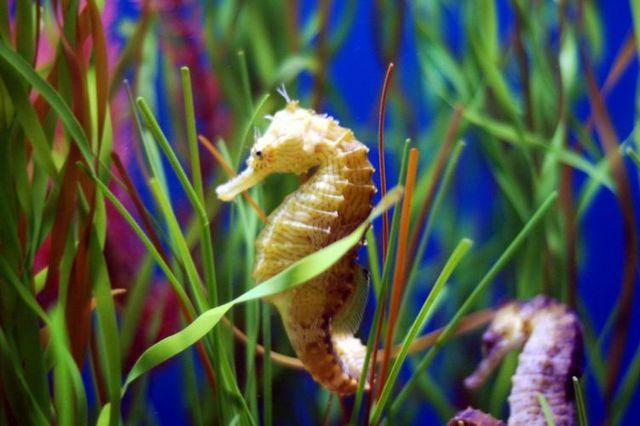
\includegraphics[scale=1.45]{SeaHorse} \includegraphics[scale=0.045]{GreenSeaTurtle} }
\caption[Importance of seagrass for marine life]{Seahorse (left) uses seagrass for their habitat and Green sea turtle (right) grazing on seagrass leaves, pictures taken from \textit{amagintheseaworldpress.com} and  \textit{mikegil.com} respectively  }
\end{figure}

The relative safety of seagrass meadows from strong water current provides an ideal environment for the female fishes to lay and hatch their eggs \cite{rooker98}. The safety of seagrass meadows are also useful for the juvenile fish and invertebrates to hide themselves from predators. Seagrass leaves are also ideal for the attachment of larvae and eggs, including those of the sea squirt and mollusk. While seagrasses are ideal for juvenile and small adult fish for escaping from the larger predators, many infaunal organisms (animals living in soft sea bottom sediments) also live within seagrass meadows. Species such as clams, worms, crabs and echinoderms, like starfishes, sea cucumbers, and sea urchins use the buffering capabilities of seagrasses to provide a refuge from strong currents. The dense network of roots established by seagrasses also helps deter predators from 
digging through the substratum to find 
infaunal prey organisms. Seagrass leaves provide a place of anchor for seaweeds and for filter-feeding animals like bryozoans, sponges, and forams as well.

Seagrasses help in trapping fine sediments and particles that are suspended in the water column, which increases water clarity. When a sea floor area lacks seagrass communities, the sediments are more frequently stirred by wind and waves, decreasing water clarity, affecting marine animal behavior and generally decreasing the recreational quality of coastal areas. Seagrasses are also known to sequester $C O_2$ \cite{duarte2005}, mix and recycle the nutrients necessary for life of its inhabitants. Seagrasses also work to filter nutrients that come from land-based industrial discharge and stormwater runoff before these nutrients are washed out to sea and to other sensitive habitats such as coral reefs.
%However these ecosystems are disappearing at an alarming rate (average $7\%$ since 1990).

The primary requirement for active marine eco-systems are presence of sunlight and a mechanism to mix and transport the nutrients. Since sunlight can penetrate only near the surface of water, the sea-shores are ideal place for rich marine ecology. One of the other important factor in proliferating the marine ecology near the ocean shores is the presence of regular wave and tides which constantly stir the region. This mechanism which is not present in most lakes. Despite shallow average depth of lakes (e.g. average depth of Lake Erie is 18.6 m and that of lake Chad is 4 m) with plenty of sunlight, lakes are not able to support a rich ecology as compared to the coastal shore due to absence of tidal mixing. The coastal oceans are about 10 times as productive as the lakes \cite{nixon1988}. Along with marshes and mangroves, seagrasses meadows rank the highest in terms of biomass production.
\newline
%\newline
The ability of seagrass meadows to engineer the habitat for effective ecosystems is directly related to its ability to influence hydrodynamic processes. This requires a balance between
two competing requirements such as flow should be sufficiently slow so that species don't get flushed along with the water, but not stagnant and thus allowing the nutrients and other material to be transported by the flow. It is widely believed that many systems, including seagrass, rely on the flow for the transportation and mixing of nutrients, pollens, sperms etc. A simple estimate of mixing-strength in absence of any flow instability can be estimated to help us understand the importance of existence of flow instability. A typical seagrass patch extend from $10^2$ m to $10^3$ m with a typical flow speed of $0.1$ m/s to $1$ m/s, indicating that any tracer particle carried by the flow would take about $\tau = 10^2-10^4$ s to cross the patch. In the absence of any flow instability mean flow is horizontal and vertical transportation and mixing of material can happen only through turbulent diffusivity $\kappa =  0.1 U d$, where $ U \approx 1$ cm/s is the mean flow in canopy, and $d \approx 1$ cm is 
characteristic 
length scale of plant such as its diameter or leaf width \cite{Nepf99}. This estimate indicates that transportation of material above the grass bed can only penetrate about $\sqrt{\kappa \tau} = 3-30$ mm, compared to the canopy height of 10-100 cm. However, in the presence of flow instability even a modest $10\%$ conversion of horizontal flow to vertical velocity results in penetration length scale of about 10-1000 cm. Indeed, It is widely believed that the phenomenon of large amplitude coherent oscillation of marine grass, known as \textit{Monami} is a result of flow instability, much like coherent waves commonly observed on terrestrial grass field, known as \textit{Honami} in strong wind \cite{Inoue55_1, Inoue55_2, Raupach96, Delangre06}. While the two cases seems superficially similar, there are major difference such as atmospheric flow is essentially unbounded. Another major difference between the two is the considerable difference of stiffness of canopies.
\newline
%from   assuming the plant diameter to be  exhibit rich set of dynamical behavior due to their interaction with the flow of water. The hydrodynamic processes resulting from these behavior are known to influence
%number of environmental processes such as transportation and mixing of sediments, contaminants, dissolved oxygen etc. One such response of submerged grass
%vegetation in response to unidirectional steady current is the large amplitude coherent oscillations, known as \textit{Monami}, which have been observed in laboratory(Ikedea, Nepf) as well as in observation of seagrass meadows in field studies (Kensworthy, Grizzle). Transportation and mixing of nutrients in dense canopies are known to be dominated by the phenomenon of \textit{Monami} which directly influences biomass production of marine plants as well as inhabitants of grass bed. 
%Similar phenomenon of large amplitude coherent oscillations are also observed for terrestrial canopies which are known as \textit{Honami}. A crucial difference between the atmospheric and aquatic flow is that the atmospheric are essentially unbounded vertically.
\section{Previous Work}
While considerable research is done to understand the phenomenon associated with atmospheric flows through terrestrial canopies, research for the case of flow through aquatic vegetation is not prevalent. Evidence of the effect of aquatic plants on unidirectional flow emerges from various study of research groups interested in conveyance of water through vegetated canals \cite{kouwen93}, the cycling of particulate and dissolved matter etc. One such systematic study on the topic of blue mussels larvae settlement attributed the excess presence of blue-muscel larvae on the tip of grass to the presence of \textit{Monami} \cite{Grizzle96}. The most notable research work related to \textit{Monami} are laboratories study of open channel flow through flexible and rigid canopies by Nepf and Ghisalberti \cite{Ikeda96,Ghisal02}, which shows existence of coherent eddies propagating on canopy top. 
\begin{figure}
 {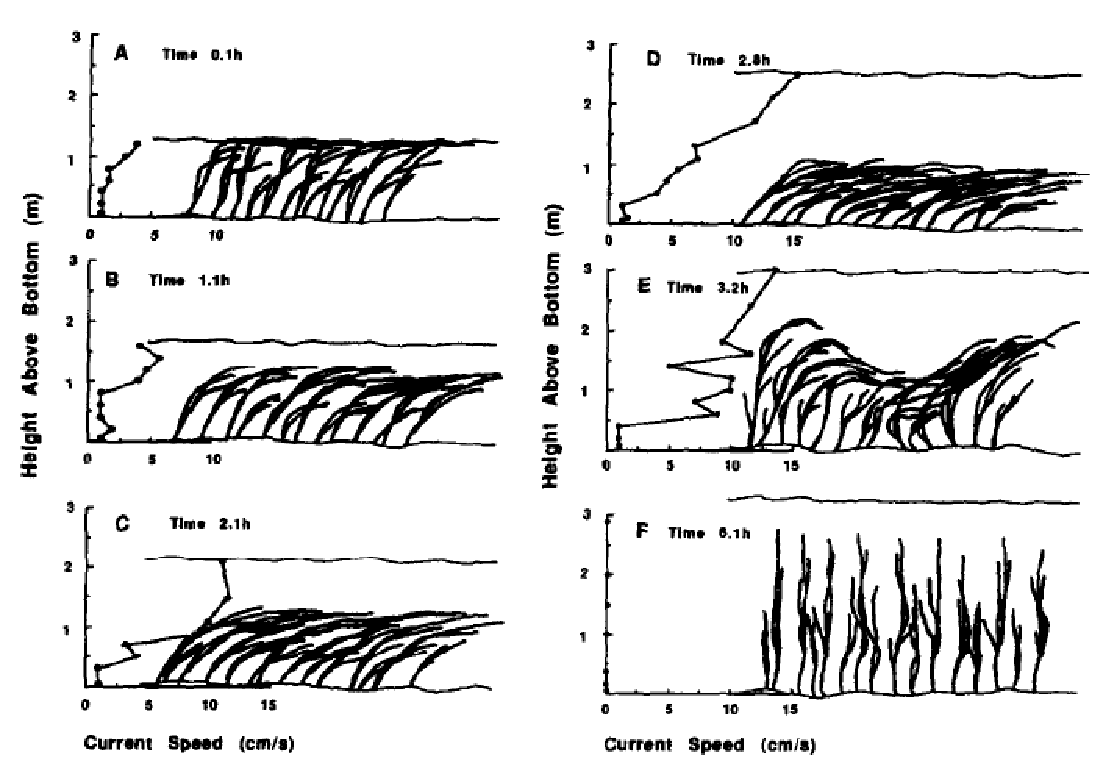
\includegraphics[scale=0.72]{Grizzle}}
 \caption[Experimental observation of \monami]{Sketches made by Grizzle, et al. \citep{Grizzle96} from direct observations of eelgrass blades in the mouth of the Jordan river, ME, USA, in response to a tidal
 flow through half a tidal cycle. The horizontal velocity profile is also plotted with each of the sketches. The grass spontaneously starts to wave in frame E, when the flow 
 speed exceeds a threshold of 10-15 cm/s.}
 \label{GrizzleFig}
\end{figure}

The current explanation of \textit{Monami} is proposed by Ghisalberti and Nepf \cite{Ghisal02,Nepf00}, which is inspired by the work of Raupach \cite{Raupach94,Raupach96} for the case of terrestrial canopies. The work of Raupach \cite{Raupach94,Raupach96} is based on Kelvin-Helmholtz (KH) instability of free shear flow. According to this mechanism, the essential role of vegetation is to exert drag on the flow slowing it down, and giving rise to velocity differential between the canopy and the region above it. This so called shear layer profile is expected to be hydrodynamically unstable to KH instability and break down into coherent vortices. The flexibility of grass blades merely aids in visualizing these vortices by deforming as they are advected past by the flow.
According to this shear layer model, the velocity profile of flow through vegetation can be approximated to a characteristic shear like profile - `` one where shear does not arise from the boundary condition'' e.g. $U(y) = \Delta U[1+\tanh(y/\delta)]$, in an approximately unbounded domain $-\infty < y< \infty$. Using the shear layer thickness $\delta$ determined by fitting to the measured mean velocity profile (e.g. see \ref{basicflow} ), the frequency predicted by KH instability agrees well with the laboratories observations.

However, several aspects of existing theory remain unexplained. First, existing theory assumes the existence of shear layer near the grass top due to presence of drag discontinuity in the vertical direction caused by the vegetation; however, it does not take into account the effect of vegetation drag while considering instability analysis of shear flow, i.e., the shear layer is treated as a free shear as far as instability analysis is concerned. In other words, the assumption of instability of perturbation to shear layer through a mechanism of Kelvin-Helmholtz relies on absence of any interaction between the flow perturbation and vegetation drag, making shear layer an inconsistent theory. Second, classical free shear flow is known to be unstable for all the Reynolds number. On the contrary, a threshold flow speed is observed in the field for the grass to spontaneously wave \cite{Grizzle96}; below this threshold speed the grass bends steadily in response to steady current. This threshold speed corresponds 
to a  critical Reynolds number $\approx O(1000)$, based on turbulent viscosity. 
 
Another closely related problem is the flow around emergent patches, which have many similarities with the flow through submerged vegetation. The flow around emergent patches develops a strong shear in the velocity profile in the horizontal direction near the patch boundary similar to the one developed in the flow through submerged vegetation near the grass top in the vertical direction. The primary reason for the existence of a region of strong shear near the patch boundary in case of flow around emergent vegetation and near the grass top in case of flow through submerged vegetation is the discontinuous drag
experienced by the flow due to presence of obstruction in the horizontal and vertical direction, respectively. However, the two cases have some differences as well. One difference between these two cases is the presence of isotropic drag in case of flow around emergent patches as compared to the anisotropic drag experienced by the flow through submerged vegetation.
The presence of isotropic drag in case of flow through emergent patch can be understood by observing that both the dominant component of flow is in the horizontal direction, hence, across the vegetation. In contrast, in the case of flow through submerged vegetation only one of the dominant components of the flow is across the  vegetation, the other component is along the vegetation and it experiences negligible drag. An analysis of shallow flow around emergent patches has been carried out by White $\&$ Nepf \cite{White07}. However, in their analysis they also 
assumed steady profile to be hyperbolic 
tangent in the horizontal direction and the flow domain to be infinite.


%They also assumed isotropic drag due to vegetation and bed friction. Since both the dominant component of flow velocity are in the same plane as bed, we expect both these component to experience similar drag due to vegetation. However for flow through submerged vegetation one of dominant component is perpendicular (vertical velocity in Figure ~\ref{GrizzleFig}) to the bed plane and hence experience negligible drag as compared to the other component which is in the plane (horizontal velocity in Figure ~\ref{GrizzleFig}).

These drawbacks of existing theory suggest that both the flow through submerged vegetation and the flow around emerged patches require further investigation for a better understanding of the phenomenon.
\section{Our Approach}
In this study, we have developed a two dimensional mathematical model for the linear stability analysis of flow through submerged vegetation. We used continuum approximation for the drag experienced by flow due to presence of grass. A linear stability analysis of this model shows that a competition between destabilizing effect of shear and stabilizing effect of drag dissipation leads to a critical flow condition characterized by Reynolds number, above which flow becomes unstable, leading to \textit{Monami}. Our linear stability analysis predicts existence of two different modes of flow instability which we termed as Mode 1 and Mode 2. Flow instability associated with Mode 1 is found to be localized on the length scale of shear layer formed near the canopy top, whereas Mode-2 is represented by the flow instability on the scale of full water column. We found that Mode 1 shares characteristics of Kelvin-Helmholtz instability such as instability on the scale of 
shear layer thickness but is found to have significant differences as well. The prediction of critical Reynolds number and waving frequency associated with \textit{Monami} is found to compare well the experimental observations. All the experimental data we have found so far corresponds to grass density at which we are unable to distinguish if the flow instability are due to Mode 1 or Mode 2.

We have also performed full numerical simulation of the mathematical model presented in equation \eqref{averaged_eq}, and compared the prediction of the linear stability analysis such as growth rate, wavelength and the resultant frequency of dominant mode with the solution of equation \eqref{averaged_eq} in section 4.2.

In chapter 5, we have also shown results from the linear stability analysis pf flow around emergent vegetation. Our calculation indicate that due to presence of isotropic drag, the flow instability associated with Mode 1 experiences significant dissipation, and is not observed in the limit of asymptotically large grass density. %However, at the grass density corresponding to the lab scale experiments Mode 1 and Mode 2 are not distinguishable from each other. 

%\lipsum[21-40]

\nocite{Lax1956,Cooley1965,Banach1924}

\clearpage{\pagestyle{empty}\cleardoublepage}

\chapter{Mathematical Model}
Given the range of length scales in the canopy (leaf thickness $<$ 1mm, leaf width $\sim$ 1cm, canopy height $\sim 1m$, vegetation patch $10^2-10^3 m$), a fully resolved direct numerical solution is challenging and unnecessary. We instead exploit this separation of length scale between the canopy scale and its microstructure, and resort to modeling the aquatic vegetation as a homogenized multiphase medium which occupies no volume but exert drag on the fluid flow.
Because the leaves are wide but thin , the volume fraction of vegetation is less than $10\%$ \cite{chandler96} in the densest of seagrass canopies, and dominant interaction of vegetation with the surrounding water is by exerting a drag on the flow. Hence to leading order, we ignore the space occupied by the grass in the fluid mass and momentum balance. In our model, vegetation is represented as a continuum field $h(x,t)$. 

%Further, lab scale experiments have shown that flow instability and resulting flow structure leading to monami are present even when the flexible grass is replaced with rigid dowels \cite{Ghisal02, Nepf06}. Therefore to develop essential mathematical model we assume grass to be rigid and oriented vertically (along y direction) on average. Since the flow structure leading to monami is dominantly 2 dimension, we assume a two dimensional model for simplicity of calculation. In our mathematical model vegetation is assumed to be sufficiently dense so that drag exerted by the grass can be modeled as a continuum field. 
The governing equation of flow in and above the grass can be represented by the fluid continuity equation incorporating the mass conservation and fluid momentum equation. The equation for incompressible fluid can be expresses as
\begin{equation}\
\begin{split}
  \grad \cdot {\bu}&=0, \\
 \rho \left[ \frac{\partial {\bu}  }{\partial t}+  {\bu} \cdot \grad \bu  \right ] &= - \grad{p} +\mu \grad^2\bu ,
\end{split}
\label{NavierStokes}
\end{equation}
where $\bu$ is velocity field, $\mu$ is molecular viscosity of fluid , $\rho$ is fluid density and $p$ is the pressure field.
For a typical flow in vegetation, the Reynolds number for flow on the scale of leaf is $O(1000)$, hence a typical flow in presence of vegetation can be treated as a turbulent flow. In order to obtain equations for mean flow, we use analysis similar to Pedras $\&$ de Lemos \cite{Pedras00}, we first average the flow over a time interval $\tau$, which is longer than the vegetation scale velocity fluctuation time, then perform spatial averaging over an area $A$, where $A$ is much larger than cross sectional area of grass. Denoting 
overbar to represent the time averaged properties and the angel brackets to denote the spatially averaged properties, for any quantity of interest, represented here by $\phi$ such as velocity, pressure etc.
  \[ \bar{\phi}(x,y,z,t) = \frac{1}{\tau} \int_{t}^{t+\tau} \phi  \, dt, \hspace{1.cm}  \langle \bar{\phi}\rangle = \frac{1}{A} \int_{A} \bar{\phi}  \,dx \,dz, \]
  \[\phi = \bar{\phi}+\phi^{'}, \hspace{1.cm}  \bar{\phi} = \langle \bar{\phi} \rangle \ +\phi^{''}, \]
 where $\bar{\phi}$ denotes temporal average, $\langle \bar{\phi} \rangle$ denotes temporally and spatially averaged quantity, $\phi^{'}$ denotes temporal fluctuation and $\phi^{''}$ denotes spatial fluctuation. Here $x$ and $z$ represents co-ordinates in the horizontal plane. Upon performing temporal averaging of Navier-Stokes and fluid continuity equation, we arrive at the following equations for fluid continuity and momentum balance.
 \begin{equation}
 \begin{split}
 \frac{\partial \bar{u_i} }{\partial x_i} &=0, \\
 \rho \left[ \frac{\partial  \overline{u_i}  }{\partial t}+  \overline{u_j}  \frac{\partial  \overline{u_i} }{\partial x_j} \right ] &= -\frac{\partial  \bar{p}   }{\partial x_i} + \mu \frac{\partial^2  \overline{u_i}  }{\partial x_j^2} - \rho \frac{\partial  \overline { u_i^{'} u_j^{'} }  }{\partial x_j}, 
 \end{split}
 \end{equation}
 and further spatial averaging gives,
  \begin{equation}\label{averaged_eq}
  \begin{split}
  \frac{\partial \langle \bar{u_i} \rangle}{\partial x_i}&=0, \\
 \rho \left[ \frac{\partial \langle \overline{u_i} \rangle }{\partial t}+ \langle \overline{u_j} \rangle \frac{\partial \langle \bar{u_i} \rangle}{\partial x_j} \right ] &= -\frac{\partial \langle \bar{p} \rangle  }{\partial x_i} + \mu \frac{\partial^2 \langle \bar{u_i} \rangle }{\partial         x_j^2} + \frac{\partial \langle \bar{\tau_{ij}} \rangle }{\partial x_j} -D_i.
 \end{split}
 \end{equation}
 Where $\tau_{ij}=-\rho \langle \overline{u_i^{'} u_j^{'}} \rangle  -\rho \langle{ \overline{u_i}^{''} \overline{u_j}^{''} } \rangle  $ is macroscopic shear stress tensor, which consists of Reynolds stresses ($ -\rho \langle \overline {u_i^{'} u_j^{'}} \rangle $) due to temporal fluctuation and dispersive stresses ($ -\rho \langle{ \overline{u_i}^{''} \overline{u_j}^{''} } \rangle $) due to spatial fluctuation. The drag force $D_i(x,y) = \langle \frac{\partial \overline{p}^{''}}{\partial x_i} \rangle - \langle \mu \frac{\partial^2 \bar{u_i}^{''} }{\partial x_j^2} \rangle $ is resistance due to vegetation, the sum of form and viscous drag over the averaging scale, which is zero above the vegetation, i.e. $D_i = 0 $ for $y>h(x,t)$. 
 %\begin{equation}
 % D_i = \langle \frac{\partial \overline{p}^{''}}{\partial x_i} \rangle - \langle \mu \frac{\partial^2 \bar{u_i}^{''} }{\partial x_j^2} \rangle
 %\end{equation}
 
 Both molecular stress ($ \mu\ \del u_i / \del x_j $) and dispersive stress($-\rho \langle \bar{u_i}^{''} \bar{u_j}^{''} \rangle $) are negligible compared to Reynolds stress ($-\rho \langle\bar{ u_i^{'} u_j^{'} } \rangle $). The former is usual assumption in analysis of a turbulent flow, such as flow in vegetation and the latter can be understood by observing that the
 lateral dimensions of canopy elements are much smaller than the canopy height so that the correlation between spatial deviation of both components of velocity on horizontal plane is small \cite{Raupach94,Raupach96}. With this assumption the equation can be further simplified into,
 \begin{equation}\label{averaged_eq2}
  \begin{split}
  \frac{\partial \langle \bar{u_i} \rangle}{\partial x_i}&=0 ,\\
 \rho \left[ \frac{\partial \langle \overline{u_i} \rangle }{\partial t}+ \langle \overline{u_j} \rangle \frac{\partial \langle \bar{u_i} \rangle}{\partial x_j} \right ] &= -\frac{\partial \langle \bar{p} \rangle  }{\partial x_i} -\rho \frac{\partial \langle \bar{u_i^{'}u_j^{'}} \rangle }{\partial x_j} -D_i .
 \end{split}
\end{equation}
In this work, we parametrized the Reynolds stress by an eddy viscosity, i.e., 
\[ -\rho \langle u_i^{'} u_j^{'} \rangle = \mu \left(\frac{\del \bar{u_i} }{\del x_j} + \frac{\del \bar {u_j} }{\del x_i}  \right) .\]
In a real grass canopy, the measured value of eddy viscosity is found to vary with depth in the water column \cite{Nepf04}. However, in this work, in-order to develop essential mathematical model we have used a constant representative value of eddy viscosity throughout the water column.
From now onwards, $\mu$ stands for eddy viscosity rather than molecular viscosity. With this simplification, equation \ref{averaged_eq2} further simplifies into,
 \begin{equation}\label{averaged_eq3}
  \begin{split}
  \frac{\partial \langle \bar{u_i} \rangle}{\partial x_i}&=0, \\
 \rho \left[ \frac{\partial \langle \overline{u_i} \rangle }{\partial t}+ \langle \overline{u_j} \rangle \frac{\partial \langle \bar{u_i} \rangle}{\partial x_j} \right ] &= -\frac{\partial \langle \bar{p} \rangle  }{\partial x_i} +\mu \frac{\partial^2 \langle \bar{u_i} \rangle }{\partial x_j^2} - D_i .
 %\rho C_N d N_g \langle \overline{u_i}\rangle |\langle \overline{u_i} \rangle|
 \end{split}
\end{equation}
Which is similar to Navier-Stokes equation with molecular viscosity replaced by a constant eddy viscosity, with an extra drag term due to presence of vegetation. From now onwards we will drop angle bracket and over bar for notational simplicity.
\begin{equation}\label{averaged_eq}
\begin{split}
  \grad \cdot {\bu}&=0, \\
 \rho \left[ \frac{\partial {\bu}  }{\partial t}+  {\bu} \cdot \grad \bu  \right ] &= - \grad{p}  +\mu \grad^2\bu - \mathbf{D} .
\end{split}
\end{equation}
When the Reynolds number of the flow on the microstructure and molecular viscosity is small, the drag force $\mathbf{D}$ can be modeled according to Darcy's law $\mathbf{D} \propto \bu$. While there is no generic way to model the drag force when Reynolds number on microstructure is large ( O(100-1000) ), general principals of high-Reynolds number flows guide us towards a phenomenological model for drag. Firstly, in this range of Reynolds number, the flow separates from grass blade, forming a wake. Therefore, it is reasonable to expect the drag to scale with dynamic pressure $\rho \bu_r^2$, where $\bu_r$ is the relative velocity between the fluid and the grass blade. Moreover, we assume that the drag is anisotropic, since the flow across the grass blade is expected to experience more drag than the flow along the glass blade. Mathematically, the drag law uses projection of relative velocity along the blade and normal to the blade as.
\begin{equation}
 \bu_N = \bu_r.\bn,\hspace{0.5cm} \bu_T = \bu_r.\bt,\hspace{.5cm} \mathbf{D} = -\rho d(x,y)\left( C_N \bu_N |\bu_N|\bn + C_T \bu_T |\bu_T| \bt \right),
\end{equation} 
where $C_N$ and $C_T$ are drag coefficient in the normal and tangential directions respectively, $N_g$ is the grass number density, $d(x,y)$ is average grass diameter at location specified by co-ordinates $(x,y)$, $\bt$ is average unit vector tangent to the grass element at $(x,y)$, and $\bn$ is average unit vector normal to the grass blade at $(x,y)$. In a real grass canopy $C_T \ll C_N$. In order to develop essential mathematical model we take $C_T=0$ in this analysis. So,
\begin{equation}
 \mathbf{D} = -\rho d(x,y) C_N \bu_N |\bu_N| \bn, \hspace{.5cm} %\text{for the flow through submerged grass bed.}
\end{equation}
\text{for the flow through submerged grass bed.} In the case of flow around emergent vegetation both dominant components of the flow are in the horizontal direction and hence across the vegetation, which suggests that vegetation drag in case of flow around emergent vegetation can be modeled by an isotropic drag, i.e,
\begin{equation}
 \mathbf{D} = -\rho d(x,y) C \bu |\bu| ,% \hspace{.5cm} \text{for the flow around emergent vegetation,}
\end{equation}
\text{for the flow around emergent vegetation.} Where $C$ is the drag coefficient for flow around emergent vegetation.
%The orientation of grass blade can be obtained by solving force and torque balance equation together with a constitutive relation relating bending moment $M$ to the curvature $\kappa$
%\begin{figure}
% \centerline{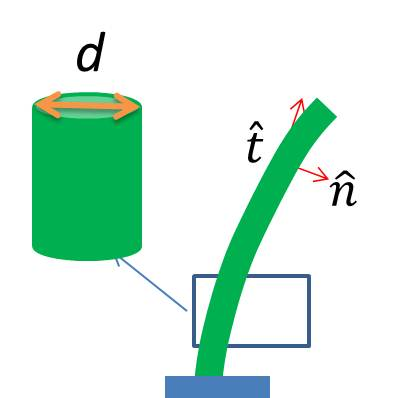
\includegraphics[width=2.8cm, height = 2.8cm]{Grass_mod1}\hspace{2.5cm} 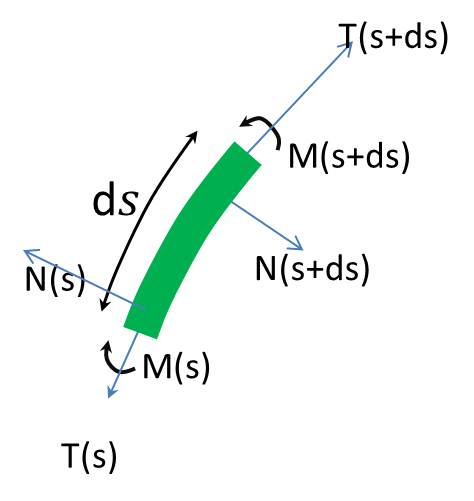
\includegraphics[width=3.cm,height=3.cm]{Grass_mod2}}
% \caption{Schematic of mechanics of individual grass blade deformation}
% \label{grass_blade_deformation}
%\end{figure}
%\begin{equation}
% \frac{\partial}{\partial s}\left( T\bt + N\bn \right)+\mathbf{f_d}+\mathbf{f_{buoy}} =0 \hspace{.5cm} \frac{\partial M}{\partial s} -N =0 \hspace{.5cm}  M = B\kappa
%\end{equation}
%Where $s$ is the arc-length along the grass blade, $\mathbf{f_{buoy}}$ is the force of buoyancy on the submerged grass blade and $\mathbf{f_{d}}$ is the drag force per unit length experienced by the grass blade. Since the marine grass blades are extremely flexible so we can safely ignore the role of bending stiffness in determining the orientation of grass blade,  which results in solving a simplified equation, subject to inextensiblity of the grass blades. 
%\begin{equation}
%  \frac{\partial}{\partial s} T\bt +\mathbf{f_d}+\mathbf{f_{buoy}} =0
%  \label{orientation_eq}
%\end{equation}
%The equation \eqref{orientation_eq} together with the equation \eqref{averaged_eq} can be solved subject to appropriate boundary condition to predict flow structure and grass orientation.
%Although {\monami} is manifested in the motion of grass, the drag exerted by the vegetation on the flow is central to flow instability leading to {\monami}. Since the instability and resulting flow structures leading to monami persist even when the flexible grass mimics are replaced with the rigid dowels \cite{Ghisal02,Nepf06}. Therefore, to develop essential mathematical model, we assume grass blade to be rigid and on average oriented vertically.

Boundary condition for \eqref{averaged_eq} include no-shear ( $u_y=0$ ) and no normal velocity ($v=0$) on the both bottom surface and top surface.
In real flow the true boundary condition at the bottom surface is no slip velocity and no normal velocity; however, the boundary layer formed due to no slip condition is so thin ($\approx 0.5 cm$) that it's hardly visible in experiments as can be seen from the experimental data of \cite{Nepf04} in Figure \ref{basicflow}. The presence of thin boundary layer near the grass bed can also be understood by observing that in the limit of dense vegetation, the shear stress exerted by the bottom surface is expected to be negligible compared to the vegetation drag \cite{Nepf04}, hence the bottom boundary condition can be approximated by no shear ($u_y(0)=0$) and no normal flow ($v(0)=0$) condition.
On the top surface, a rigid lid condition ( no shear and no normal velocity ) or free surface is suitable. In order to model free interface we have used no shear at top as well. Since changes in water surface elevation due to presence of {\monami}  is small compared to the depth of water channel, we can approximate the top surface by no normal flow ($v(2H)=0$) as well.  %The no shear condition arises because, for dense vegetation the shear stress exerted by the bottom surface is expected to be negligible compared to the vegetation drag. On the top surface, a rigid-lid condition (no shear and no normal velocity) or a free surface condition is suitable. In this analysis we have used rigid-lid condition on the top surface.
 %The prediction of mean velocity made based on these condition agrees well with the experiments (e.g see Figure ~\ref{basicflow} ). 
%\lipsum[61-80]

\clearpage{\pagestyle{empty}\cleardoublepage}
\chapter{Linear stability analysis for flow through submerged vegetation}
The usual response of submerged grass to steady current is to remain bend steadily in some fixed configuration. However, above certain flow velocity the grass beds shows coherent large amplitude oscillation as well, such response of time dependent large amplitude oscillation exhibited by the vegetation under the influence of otherwise steady current is thought to be understood as a result of hydrodynamic instability. Lab scale experiments also show that the flow structures resulting into {\monami} are present even when the flexible grass is replaced by rigid dowels \cite{Ghisal02,Nepf04}, so, to develop essential understanding of flow instability leading to {\monami}, we assume grass to be rigid and oriented vertically. 
\section{Base velocity profile}
In order to understand nature of the flow instability associated with \monami, we first calculate the fully developed steady solution $\bu = U(y)\boldsymbol{\hat{x}}$ of ~\eqref{averaged_eq} driven by constant pressure gradient $dP/dx$, and use it to non-dimensionalize the mathematical model. The momentum balance \eqref{averaged_eq} for steady $U(y)$ simplifies to
\begin{equation}
\begin{split}
 -&\frac{dP}{dx}+\mu U''(y) -S(y) \rho C_N d N_gU |U| =0,\\
 &S(y) = 1, \hspace{2cm} 0<y<\hg,\\
 &S(y) = 0, \hspace{2cm} \hg< y< 2H.
\label{base_equ}
\end{split}
\end{equation}
Eq. \eqref{base_equ} is solved subject to no shear at the boundaries, i.e., $U'(0) = U'(2H) = 0$.
A comparison of the steady flow profile from the solution of ~\eqref{base_equ} with experimental measurements is shown in Fig ~\ref{basicflow}.
\begin{figure}
\centerline{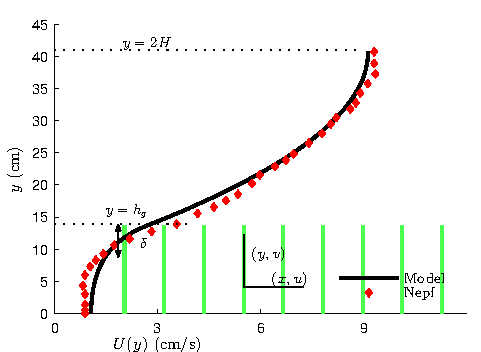
\includegraphics[scale=.99]{Grass_Base_Nepf} }
% 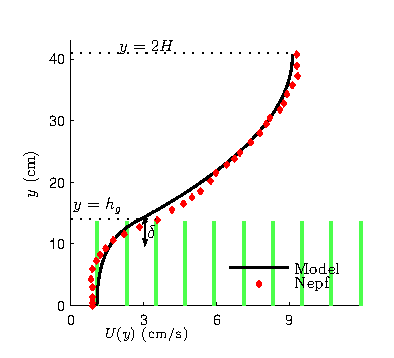
\includegraphics[width=15cm]{Grass_Base_Nepf_shear}
\caption[Comparison of experimentally measured mean velocity profile with the prediction of mathematical model]{
Schematic setup and comparison of our steady flow profile with that from the experiments in ref. \cite{Nepf04} (Case I from Table 1) %  with 1250 plants/m$^2$, plant height = 13.7$\pm 0.2$ cm and blade width of 0.64 cm)
 and its approximation with $U_0=7.28$ cm/s and $\delta = 5.02$ cm in our model. The grass extends up to $y=\hg$ in the water column of depth $2H$. 
The steady velocity profile can be decomposed into a parabolic profile in the unvegetated region, a uniform profile deep within the vegetation, and a boundary layer of thickness $\delta$ near the grass top. 
}
\label{basicflow}
\end{figure}
The profile $U(y)$ has three distinct regions.
Within the vegetation, it is approximately uniform with $ U(y) \approx U_g = \sqrt{\frac{-dP/dx}{\rho C_N dN_g}}$, which arise from the balance of the drag with the pressure gradient. 
Outside the vegetation, the velocity has a simple parabolic profile similar to a Poissueille profile, arising from the balance between pressure and viscous forces together with the free shear condition at the top surface. 
At the grass top, continuity of shear stresses results in a boundary layer of thickness $\delta$ in the velocity profile. Denoting $\ubl$ to be the velocity scale in the boundary layer, and $U_0 = {(-dP/dx)~H^2}/{\mu}$ is the velocity scale in the unvegetated region, the balance between viscous forces and vegetation drag with in grass implies $(\mu \ubl/\delta^2 \sim \rho C_N d N_g \ubl^2)$, and the continuity of shear stress across the grass top implies $(\ubl/\delta \sim U_0/H)$.
Solving for $\delta$ and $\ubl$ yields $\delta/H \sim \ubl/U_0 \sim (\Rey \Ndg )^{-1/3}$, where $\Ndg = \left(C_N d H N_g\right)$ is the vegetation frontal area per bed area, and $\Rey=\rho U_0 H/\mu$ is the Reynolds number of the flow. 
A numerical estimate of $\delta$ (estimated as $U/U_y$ at $y=\hg$) is compared with this prediction in figure \ref{Uy_base} (right). Since the existence of this boundary layer is not influenced by the boundary of the flow domain, we identify it as similar to the shear layer invoked by the Ghisalberti $\&$ Nepf \cite{Ghisal02,Nepf04}, i.e. `` one where shear does not arise from boundary conditions''.

We can also understand the scales for $U_{bl}$ and boundary layer thickness $\delta$ by integrating equation \eqref{basicflow} from $(h_g-\epsilon)$ to $2H$.
\begin{equation}
 \int_{h_g - \epsilon}^{2H} \left( -\frac{dP}{dx}+\mu U''(y) -S(y) \rho C_N d N_gU |U|\right)dy = 0 
\end{equation}
\begin{equation*}
-\frac{dP}{dx}(2H-h_g+\epsilon)+\mu (U_y(2H)-U_y(h_g-\epsilon)) -\int_{h_g-\epsilon}^{h_g} \rho C_N d N_gU |U|dy  =0
\end{equation*}
The above equation can be further simplified by observing that $U_y(2H)=0$ due to zero shear boundary condition and $U_y(h_g-\epsilon) \approx 0$ due to approximately constant velocity below the boundary layer, we also observe that $\int_{h_g-\epsilon}^{h_g} U |U| dy \sim O( U_{bl}^2 \delta )$.
%\begin{equation*}
%-\frac{dP}{dx}(2H-h_g+m\delta) - \rho C_N d N_g U_{bl}^2 m \delta \alpha  =0
%\end{equation*}
Further, since $\epsilon \ll H$ we can ignore $\epsilon$ in comparison to $2H-h_g$.
\begin{equation}
-\frac{dP}{dx}(2H-h_g) \sim O( \rho C_N d N_g U_{bl}^2  \delta )
\label{estimateDelta}
\end{equation}
In the above equation the left term $ -\frac{dP}{dx}(2H-h_g)$ is the total shear stress applied at the grass tip by flow above the canopy, which is balanced by the drag $\rho C_N d N_g U_{bl}^2 \delta $ within the boundary layer. By observing that $ U_{bl}/\delta \sim U_0/H$ due to continuity of shear stress at the grass top and $U_0 = (-dP/dx) H^2/\mu$, equation \eqref{estimateDelta} can be solved for $\delta$ and $U_{bl}$
\begin{equation}
 \delta = \beta (R\Ndg)^{-1/3} \hspace{1.5cm} U_{bl} = \frac{\delta}{H} U_0 
 \label{delta_asymp}
\end{equation}
where $\beta$ depends only on submergence ratio. For another presentation of the boundary layer analysis see Appendix A. The numerical estimate of $\delta$ (estimated as $U/U_y$ at y = $h_g$) for the experimental data of \cite{Nepf04} is shown in Figure \ref{Uy_base} (left). we have also shown the comparison of numerical estimate of $\delta$ with the prediction of \eqref{delta_asymp} on the right panel in figure ~\ref{Uy_base}.
The prediction of \eqref{delta_asymp} with the solution of \eqref{base_equ} are also shown in Figure ~\ref{base_collapse}. 

%We identify the boundary layer near the grass tip to be analogous to the shear layer \cite{Ghisal02,Nepf04} in the previous explanation of \monami.
The dependence of $\delta$ on $N_g$ gives us a way to systematically investigate the effect of the shear layer thickness on the instability mechanism.
Figure ~\ref{Uy_base} also shows that the asymptotic regime of a thin boundary layer is expected to hold for $\ReyNdg \gtrsim 100$. 
In this notation, $U_g/U_0 = (\Rey \Ndg)^{-1/2}$. 
\begin{figure}
\centerline{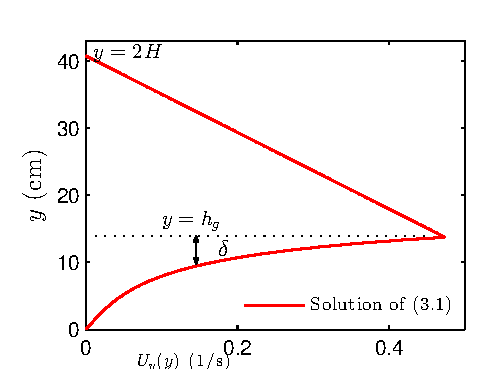
\includegraphics[scale=1.]{Grass_Base_Nepf_shear_scale} 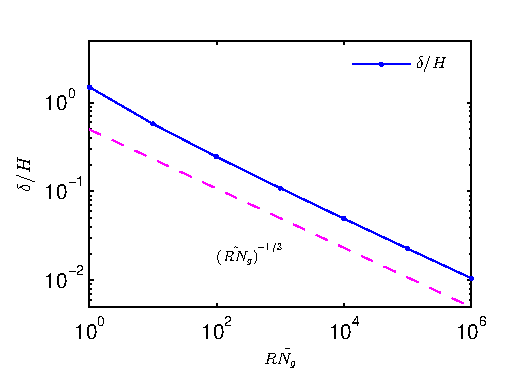
\includegraphics[scale=1.]{Grass_shear_scale}}
% 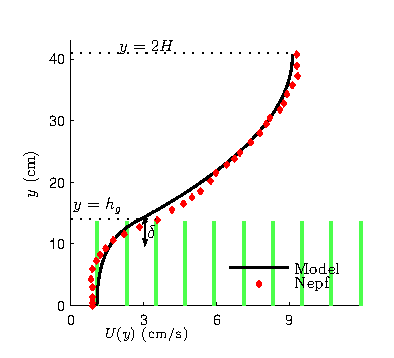
\includegraphics[width=15cm]{Grass_Base_Nepf_shear}
\caption[Numerical estimate of shear thickness for experimental data]{Graph showing numerical estimate of $\delta$ for the experimental data of \cite{Nepf04} (Case I from Table 1) from the numerical solution of \eqref{base_equ}). The dependence of boundary layer thickness (estimated as $|U/U_y|$ at y = $h_g$ from numerical solution of \ref{base_equ} on the vegetation density parameter $R\Ndg$ is shown on the right.
}
\label{Uy_base}
\end{figure}

\begin{figure}
\centerline{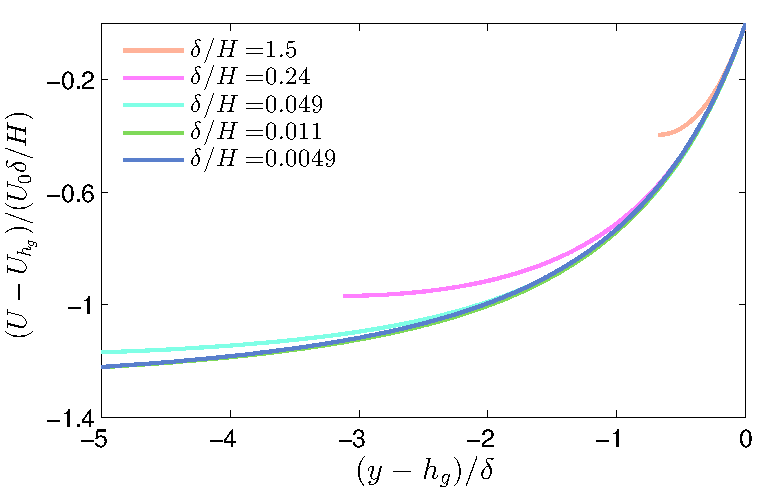
\includegraphics[]{Grass_shear_scale_collapse} }
\caption{
Collapse of velocity profile near the grass tip over boundary layer thickness $\delta$  
}
\label{base_collapse}
\end{figure}
\section{Governing equation for flow instability}
 In order to understand the nature of perturbation to the flow arising from the solution of \ref{base_equ}, we substitute $\bu = (U+\tilde{u}, \tilde{v})$, $p=P+\tilde{p}$ in ~\eqref{averaged_eq} and expand to linear order to investigate the evolution of small perturbations $(\tilde{u}, \tilde{v})$, which obey
\begin{equation}
\begin{split}
\rho(u_t+U u_x+vU_y) &= -p_x+ {\mu}\nabla^2u-2S\rho C_{N}dN_{g}Uu, \\
\rho(v_t+ Uv_x) &= -p_y+ {\mu}\nabla^2v, \hspace{0.3cm} \nabla\cdot\bu=0,
\label{LinearizedNavierStokes}
\end{split} 
\end{equation}
where the tilde are dropped for simplicity.
We non-dimensionalized these equation using half channel height $H$, velocity $U_0$, and time $H/U_0$, leading to three non-dimensional parameters, namely $\Rey$, $\Ndg$, and the vegetation submergence ratio $\hg/H$. 
We also use $\delta/H$ in lieu of $\Ndg$ to parametrize the vegetation density in order to elucidate the instability mechanism. 
Using a stream function $\psi$ with $u = \psi_{y},$  $v= -\psi_x$ to satisfy mass balance, we seek a solution of 
the form $\left(u,v,\psi \right)= \left(\hat u(y), \hat v(y), \phi(y) \right)e^{ikx+\sigma t}$. After substituting $(u,v)$ in equation \eqref{LinearizedNavierStokes} and eliminating pressure term, we obtain a modified Orr-Sommerfeld equation \cite{Drazin81,Chen97,Chu91} 
\begin{equation}
\begin{split}
\Rey^{-1}\left(D^2 -k^{2} \right)^2\phi &= \left[ \left({\sigma}+ikU\right) \left(D^2-k^2\right) -ikU_{yy}\right]\phi + \Ndg D\left(2 S U D \phi\right),
\label{Orr-somerfield}
\end{split}
\end{equation}
where $D=d/dy$. The equation \eqref{Orr-somerfield} is solved with the boundary conditions $\phi = D^2\phi = 0$ at $y=0$ and $y=2$, which are consistent with the zero shear and no normal flow at both boundary. 
The growth rate $\sigma$ for a given wave number $k$ arises as an eigenvalue that allows a non-trivial solution $\phi$ of equation \eqref{Orr-somerfield}.
\subsection{Numerical Method}
  In order to solve equation \eqref{Orr-somerfield}, we used finite difference method with $N$ equally spaced grid points $(y_i = i\Delta y, \Delta y = \frac{2}{N})$, and used second order approximation for various terms in equation \eqref{Orr-somerfield} at these grid points. We used following approximation for evaluating various derivatives appearing in equation \eqref{Orr-somerfield}
  \begin{equation}
  \begin{align}
    \left.{ D^4\phi} \right|_i &= \frac{ \phi_{i+2}-4\phi_{i+1}+6\phi_{i}-4\phi_{i-1}+\phi_{i-2} }{\Delta y^4} - \frac{\Delta y^2}{6} \left. \frac{\del^6 \phi}{\del y^6} \right |_i, \\
    \left. D^2\phi \right|_i &=  \frac{\phi_{i+1} -2\phi_i +\phi_{i-1}}{\Delta y^2} - \left. \frac{\Delta y^2}{12} \frac{\del^4 \phi}{\del y^4} \right|_i ,\\    
    \left. D\phi \right|_i &=  \frac{\phi_{i+1} -\phi_{i-1}}{2\Delta y} - \left. \frac{\Delta y^2}{6} \frac{\del^3 \phi}{\del y^3} \right|_i, \\
    \end{align}
  \end{equation}
where the terms $O(\Delta y^2)$ are truncation error to the approximation of the derivatives at the grid points.
The boundary conditions at the top and bottom surface are approximated by $\phi_0 = 0$,  $\phi_{N} = 0$ to satisfy $\phi=0$ at the top and bottom surface.
The zero shear condition at the top and bottom surface ($D^2\phi=0$) are expressed by $\phi_{-1} = -\phi_{1}$ and $\phi_{N+1} = -\phi_{N-1}$. The discontinuity of $S(y)$ across the grass tip give rise to the dirac-delta term $2\Ndg U_g D\phi_g \delta(y-h_g)$ in equation \eqref{Orr-somerfield}, where $U_g$ is velocity at the grass tip and $\phi_g$ is value of $\phi$ at the grass tip. We approximate the term with dirac-delta as $2\Ndg U_g D\phi_{g} \frac{1}{\Delta y}$.
The base velocity profile $U(y)$ at these grid points are evaluated by solving equation \eqref{base_equ}. Using these approximation we can rearrange terms in equation \eqref{Orr-somerfield} to yield
\begin{equation}
\begin{split}
A\phi &= \sigma B \phi,\\
A &= \Rey^{-1}\left(D^2 -k^{2} \right)^2\phi-ikU \left(D^2-k^2\right)\phi + ik U_{yy}\phi -\Ndg D\left(2 S U D \phi\right),\\
%\Rey^{-1}\left(D^2 -k^{2} \right)^2\phi-ikU \left(D^2-k^2\right)\phi +5 ik U_{yy}\phi &-\Ndg D\left(2 S U D \phi\right)  =\\
B &= {\sigma} \left(D^2-k^2\right) \phi,
\end{split}
\end{equation}
where the operator $A$ and $B$ are approximated at the grid points using finite difference method. This results in a finite dimensional generalized eigen-value problem, whose solution provide growth rate $\sigma$ and eigen mode $\phi$ for a perturbation of wavenumber $k$ to the base velocity profile $U(y)$. A plot of $\Re(\sigma)$ as a function of wavenumber $k$ for a base profile arising from $R=500$, $\Ndg=2$ and $h_g/(2H)=0.4$ is shown in figure \ref{GrowthRateVsK} 

\begin{figure}
 \centerline{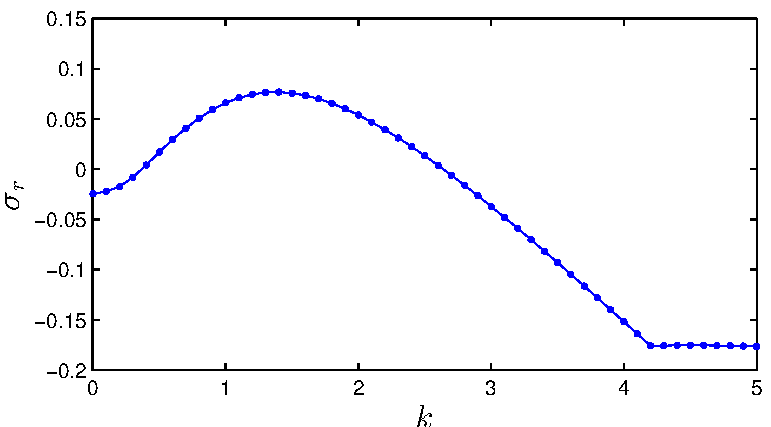
\includegraphics{GrowthrateVsK}}
 \caption[Growth rate ($\sigma_r$) of perturbation to the solution of \eqref{base_equ} as predicted by the solution of \eqref{Orr-somerfield}]{Growth rate ($\sigma_r$) of perturbation to the solution of \eqref{base_equ} as predicted by the solution of \eqref{Orr-somerfield}. The  Reynolds number, grass number density and submergence ratios are $R=500$, $\Ndg=2$ and $h_{g}/(2H) = 0.4$ respectively. }
 \label{GrowthRateVsK}
\end{figure}


%\lipsum[81-100]

\begin{figure}
  \centering
  \begin{tikzpicture}[scale=3]

  \draw [fill=red!20!white] (1,1) -- ++(0,-2) -- ++(-2,0) -- ++(0,2) -- cycle;
  \draw [fill=blue!20!white,opacity=0.4] (0,0) circle(2cm);
  \node [font={\Large\sf}] (yo) at (0,0) {Yo, yo, home slice};
  \draw[->,very thick, dashed] (yo) to [out=45,in=-45] (3,0);

\end{tikzpicture}

  \caption[Awesome picture]{Isn't this picture awesome?}
\end{figure}

\begin{figure}
  \centering
  \begin{tikzpicture}
  \draw [fill=red!70!white,circular drop shadow={shadow scale=1.05},very
  thick,rotate=45,opacity=0.7] (0,0) rectangle (3,2);


  \draw [fill=blue!70!white,circular drop shadow={shadow scale=1.05},very
  thick,rotate=135,opacity=0.7] (0,0) rectangle (3,2);
  \draw [fill=orange!70!white,circular drop shadow={shadow scale=1.05},very
  thick,rotate=225,opacity=0.7] (0,0) rectangle (3,2);
  \draw [fill=green!70!white,circular drop shadow={shadow scale=1.05},very
  thick,rotate=-45,opacity=0.7] (0,0) rectangle (3,2);
\end{tikzpicture}

  \caption[Tubular picture]{Totally tubular, dude}
\end{figure}

\clearpage{\pagestyle{empty}\cleardoublepage}

\section{Results}
\subsection{Unstable modes and critical parameters}
\begin{figure}
\begin{center}
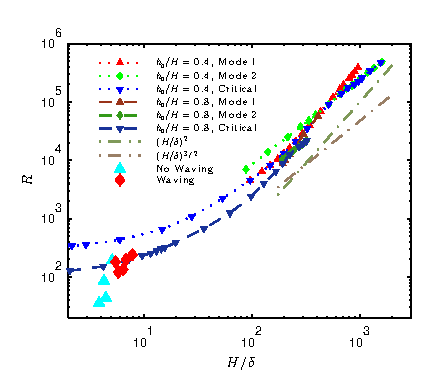
\includegraphics[scale = 0.95]{new_graph_R_vs_delta}\\
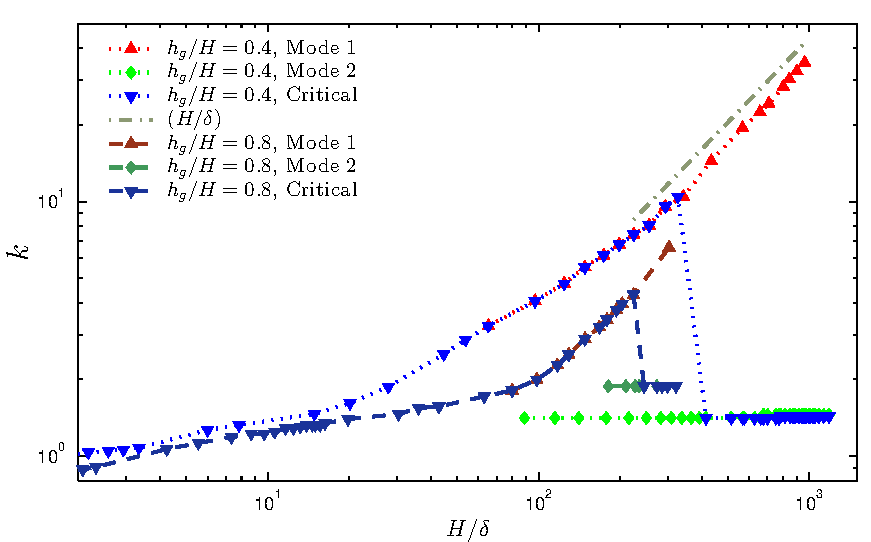
\includegraphics[scale = 0.95]{new_graph_K_vs_delta}
% 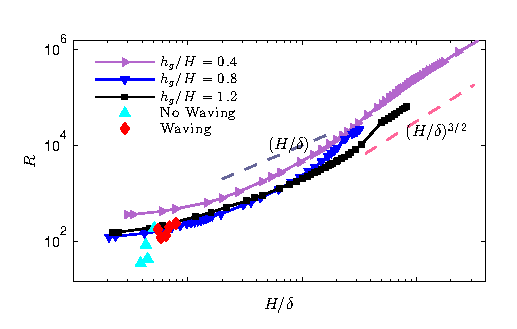
\includegraphics[width=12cm]{Critical_Re_vs_delta_noshear} \\
% \vspace{-6mm} \hspace{-5mm}
% 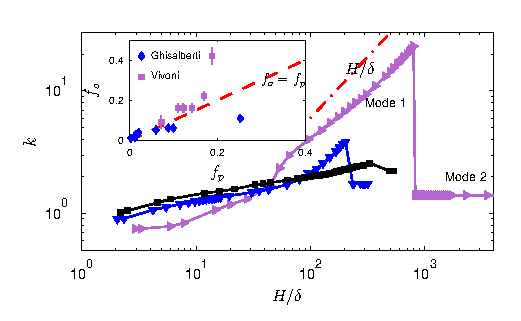
\includegraphics[width=12cm]{K_vs_shear_width_noshear}
\end{center}
\caption[ Critical Reynolds number, threshold Reynolds number for Mode 1 and Mode 2 and the corresponding marginally stable wave number for different submergence ratio]{
Critical Reynolds number, threshold Reynolds number for Mode 1 and Mode 2 (left) and the corresponding marginally stable wave number (right) for different submergence ratio as a function of vegetation density parametrized by the boundary layer thickness. 
Parameters from experiments reported by \cite{Ghisal02} to exhibit or suppress synchronous waving are also included in the left panel. 
In order to estimate the $\Rey$ for these experiments, a representative value of $\mu=0.1$ Pa~s was assumed.
}
\label{Re_vs_delta}
\end{figure}
In order to understand the critical criteria for flow instability leading to waving, we solve equation \eqref{Orr-somerfield} numerically for $\sigma$ and $\phi$, which predicts a threshold in $\Rey$, above which the flow is unstable ($\Re(\sigma)>0$) for at least one $k$. 
The dependence of this threshold $\Rey$, and the corresponding marginally stable wavenumber $k$, on $\delta/H$ and $\hg/H$ is shown in Fig.~\ref{Re_vs_delta}. We observe that the threshold $\Rey$ increases with the vegetation density which indicates a competition between the destabilizing shear in the flow and the stabilizing effect of damping due to vegetation drag.
% A similar conclusion was presented for an analogous problem (flow around an emergent (i.e., $\hg>2H$) sea grass patch), but by assuming $U(y)$ to be a tanh-profile, and neglecting the viscous term \citep{White07}.
%Previous calculations for terrestrial grass either exclude the vegetation drag in their models \cite{Raupach96}, or assume the mean velocity profile \textit{ad hoc} \citep{Raupach96,Delangre06}.
%A threshold flow condition is not reported previously either for terrestrial or submerged marine meadows.

\begin{figure*}
 \centerline{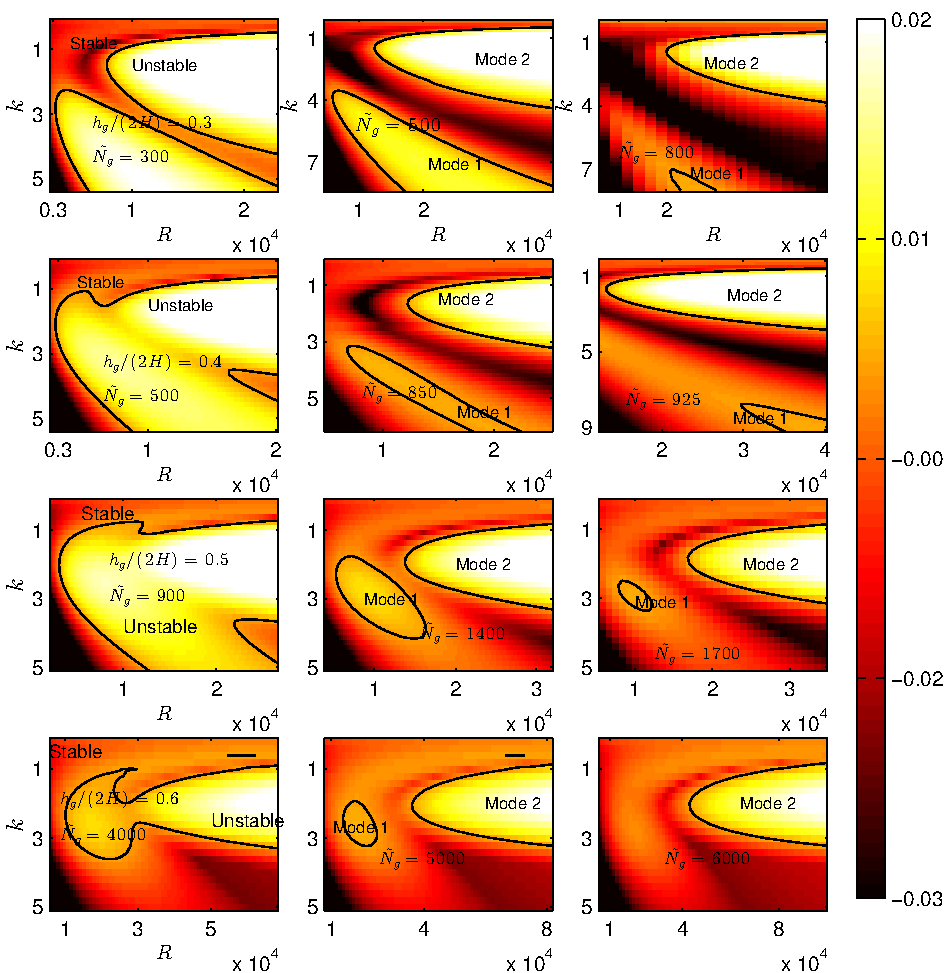
\includegraphics[]{SetAll_imgsc4}}
%\end{figure}
%\begin{figure*}
%\begin{tabular}{cccc}
%{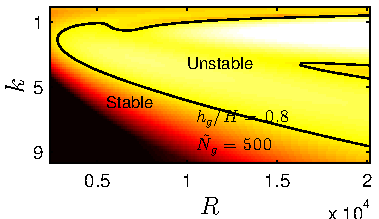
\includegraphics[height = 4cm, width = 5.8cm]{Set4_dens28_imgsc}} &
%{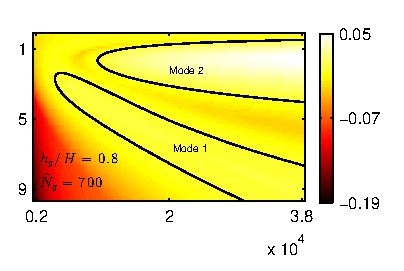
\includegraphics[scale = 0.67]{Set4_dens30_imgsc}} &
%{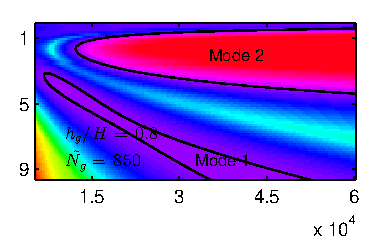
\includegraphics[height = 4cm,width = 5.8cm]{Set4_dens32_imgsc}} &
%{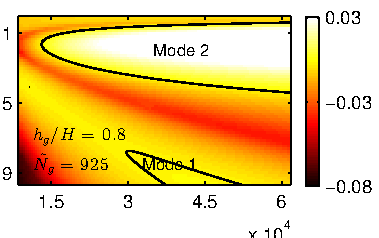
\includegraphics[height = 4.15cm,width=6.5cm]{Set4_dens34_imgsc}} \\
%{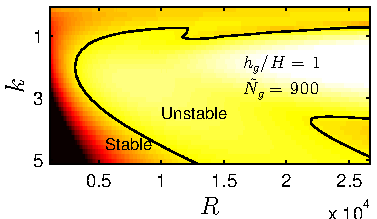
\includegraphics[height = 4cm, width = 5.8cm]{Set5_dens38_imgsc}} &
%{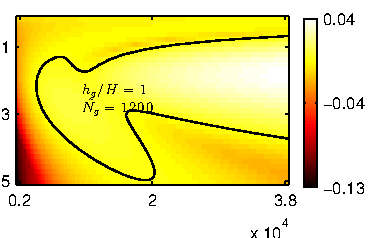
\includegraphics[scale = 0.67]{Set5_dens40_imgsc}} &
%{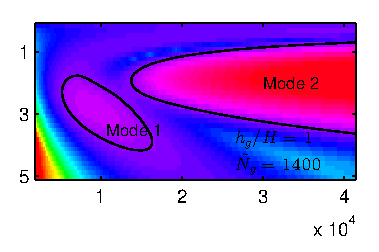
\includegraphics[height = 4cm, width = 5.8cm]{Set5_dens42_imgsc}} &
%{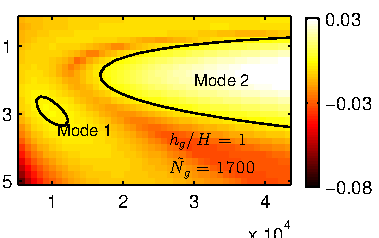
\includegraphics[height = 4.15cm,width=6.5cm]{Set5_dens46_imgsc}} \\

%{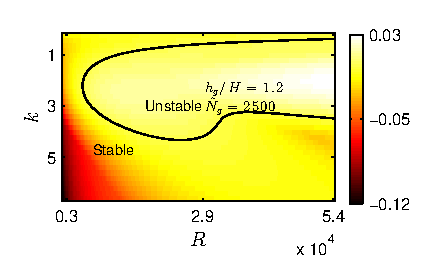
\includegraphics[scale = 0.67]{Set6_dens32_imgsc}} &
%{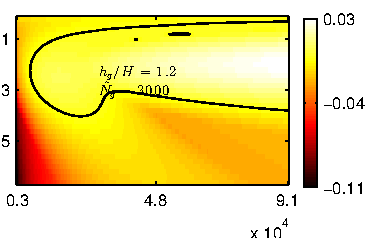
\includegraphics[scale = 0.67]{Set6_dens34_imgsc}} &
%{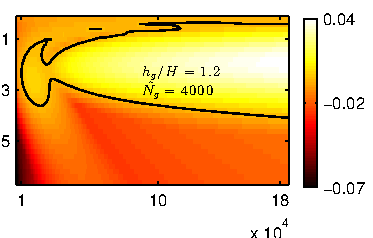
\includegraphics[scale = 0.67]{Set6_dens36_imgsc}} &
%{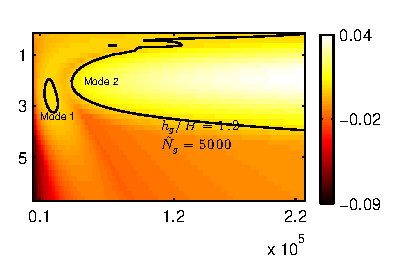
\includegraphics[scale = 0.67]{Set6_dens38_imgsc}}
%\end{tabular}
\caption[$\text{Re}(\sigma)$ and the neutral curve ($\text{Re}(\sigma)$=0) as a function of $k$ and $\Rey$]{
$\text{Re}(\sigma)$ and the neutral curve ($\text{Re}(\sigma)$=0) as a function of wavenumber and $\Rey$ for parameters shown in the corresponding panel.  
As $\Ndg$ increases, the unstable region splits into two labeled as ``Mode 1'' and ``Mode 2''. 
For $\Ndg$ below (above) a critical value, Mode 1 (Mode 2) sets the threshold $\Rey$.
}
\label{K_Re_sigma_set3}
\end{figure*}
To better understand the instability mechanism, we consider the dependence of the fastest growing wavenumber on $\delta$. Our calculation indicates that
the fastest growing wavenumber first increases proportional to $H/\delta$, but at a critical $\delta$ discontinuously jumps and remains $O(1)$ (see Fig.~\ref{Re_vs_delta}). 
To understand this behavior in greater detail, we have also plotted heat maps of $\Re(\sigma)$ as a function of $\Rey$ and $k$, for various $\hg/H$ and $\Ndg$ in Fig.~\ref{K_Re_sigma_set3}. On top of heat map of $\Re(\sigma)$, we have also plotted the contour of neutral curve $\Re(\sigma)=0$. The threshold $\Rey$ is set by the smallest $\Rey$ on this neutral curve. 
We observe that as $\Ndg$ increases, the unstable region splits into two; we refer to the region with the higher $k$ as ``Mode 1'', and the one with the lower $k$ as ``Mode 2''. 
For $\hg/H\lesssim 0.9$, the unstable region for Mode 1 recedes to higher $\Rey$, and for $\hg/H \gtrsim 0.9$, the region shrinks to zero size.
In either case, due to such behavior the most unstable mode exhibits discontinuous transition from Mode 1 to Mode 2.
So far, all the experimental data we have found corresponds to vegetation density at which the unstable region in the $\Rey-k$ has not split into two, so with these data we are unable to determine if flow instability in the lab scale experiments \citep{Nepf04} are arising due to Mode 1 or Mode 2. We numerically observe that the Mode 1 and Mode 2 exhibit different asymptotic behavior for large $\Ndg$, which distinguishes them from each other and facilitate their comparison with the KH instability mechanism.
\begin{figure}
 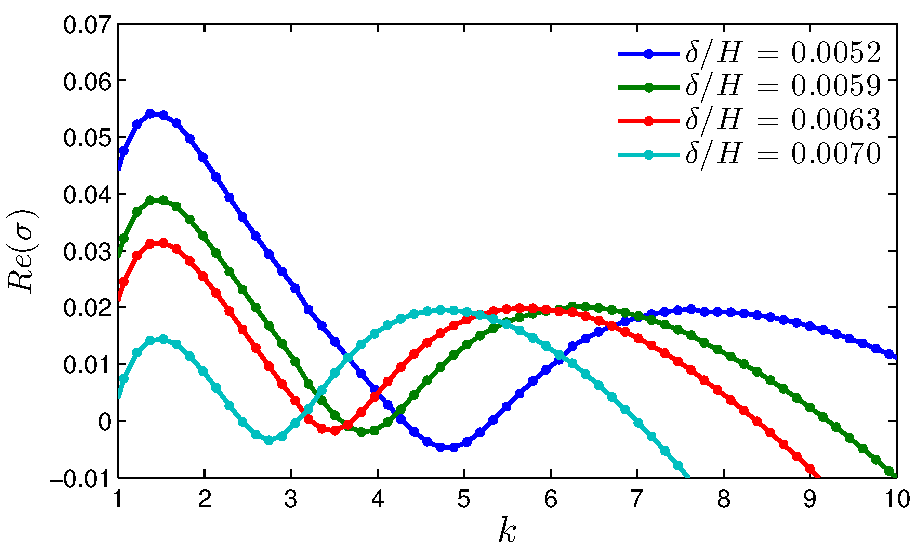
\includegraphics{K_vs_GrowthSet3}
 \caption[Growth rate for various values of $\delta/H$, as a function of wavenumber k]{Growth rate for various values of $\delta/H$, as a function of wavenumber k. The wavenumber with highest growth for Mode 2 (first peak) is always O(1), whereas for Mode 1 the wavenumber with highest growth increases as $\sim (H/\delta)$. The submergence ratio and grass number density for above graph are $0.3$ and $\Ndg = 300$ respectively.  }
 \label{K_vs_SigmaSet3}
\end{figure}


\subsection{Mode 1}
We numerically observe that the threshold Reynolds number for Mode 1 instability scales as  $\Rey \sim (H/\delta)^2$ (or $\Rey \propto {\Ndg}^{2}$). We also observe that Mode 1 is asymptotically localized to the boundary layer near the grass top, and exhibits highest growth for a perturbation of $k \sim H/\delta$ (see Fig.~\ref{Re_vs_delta}). We can understand the behavior of critical Reynolds number by performing asymptotic and dominant balance analysis in the limit $\Rey \gg 1$ and $\Ndg \gg 1$. In order to understand the behavior of critical $\Rey$, we estimate the size of various term of equation \eqref{Orr-somerfield} in the boundary layer. Observing that in the limit $\Ndg \gg 1$ and $\Rey \gg 1$, Mode 1 is localized over a length of $\delta$ near the grass top (see figure \ref{Asymptotic_mode}), we estimate $D \sim H/\delta$, we also observe that $\sigma \sim O(1)$ and $U = U_{bl} \sim \delta/H$ (see appendix A) in the boundary layer; so, the magnitude of the advection term $\left(\sigma + i k U\right)
\left(
D^2-
k^2\right) \phi$ is $ (H/\delta)^2$  (or $\Rey^{2/3} \Ndg^{2/3}$), the magnitude of the viscous term $(1/\Rey)\left(D^2-k^2\right)^2\phi$ is $(1/\Rey) (\delta/H)^{-4}$ (or $(\Rey^{1/3} \Ndg^{4/3})$), and the magnitude of the drag term $\Ndg D \left( 2 S U D \phi \right)$ is $\Ndg(H/\delta)$ or $(\Rey^{1/3} \Ndg^{4/3})$.
The advection term, viscous term and vegetation drag terms balance when $\Rey \sim (H/\delta)^2$ (or $\Rey \sim {\Ndg}^{2}$). 
%The balance between advection viscous and vegetation drag term arises when $R^{2/3}\Ndg^{2/3}  \sim R^{1/3} \Ndg^{4/3}$, i.e. when $\Rey \sim \Ndg^2$ or $R\sim (H/\delta)^2$. 




In order to gain further insight into the mechanism of Mode 1, we rescale equation \eqref{Orr-somerfield} near the grass-top using the scaling of various variables in the boundary layer, $\eta = y/(\delta/H)$, 
$U(y) = (\delta/H)\bar{U}(\eta)$ and $k = (H/\delta) \bar{k}$.
With these scalings equation ~\eqref{Orr-somerfield} simplifies to
\begin{equation}
\begin{split}
\left(\bar{D}^2 -\bar{k}^{2} \right)^2\phi &= (\Rey/\Ndg^2)^{1/3} \left[ \left({\sigma}+i\bar{k}\bar{U}\right) \left(\bar{D}^2-\bar{k}^2\right) -i\bar{k}\bar{U}_{\eta\eta}\right]\phi + \bar{D}\left(2S \bar{U} \bar{D} \phi\right),
\label{eqn:mode1asymp}
\end{split}
\end{equation}
in a region of thickness O($\delta$) near $y=\hg$, where $\bar{D} = d/d\eta$. 
Since $(\Rey/\Ndg^2)$ is the only remaining parameter in equation \eqref{eqn:mode1asymp}, we expect the mode shape and solution to converge in the limit $\Rey \gg 1$, $\Ndg \gg 1$ with $\Rey/\Ndg^2$ fixed.
Our numerical findings also confirm this expectation; we can see that the critical $\Rey$ scales as $(H/\delta)^2$ as shown in Fig.~\ref{Re_vs_delta} and the mode shapes are self-similar with length scale $\delta$, as shown in Fig \ref{Asymptotic_mode}. 

There are many similarities between the KH instability and the Mode 1 (see Table \ref{tab:comparison}). 
In case of Mode 1 the fastest growing wavenumber at the critical $\Rey$ scales as $k \propto (H/\delta)$, similar to KH instability. 
In both cases the extent of the unstable mode is also localized to the boundary layer region.
Due to the porous nature of the vegetation only a weak flow of magnitude $\ubl = U_0 \delta/H$ penetrates a thin boundary layer region $\delta$, and therefore the shear gradient $U_{yy} \sim U_0/\delta H$ is largest in this region.
The existence of strong shear gradient $U_{yy}$ in the boundary layer plays a central role in destabilizing the flow and localizing the flow instability to the boundary layer. However, there are some key differences between Mode 1 and KH instability as well. 
Our detailed description of Mode 1, given by equation \eqref{eqn:mode1asymp} highlights important differences between Mode 1 and the formulations of KH. 
KH is usually described using the inviscid Rayleigh's equation, 
\begin{align}
\left(\sigma+ikU\right) \left(D^2-k^2\right)\phi =  ikU_{yy}\phi, 
\label{eqn:Rayleigh}
\end{align}
which is not parametrized by the Reynolds number. If we describing the instability using the Orr-Sommerfeld equation, we do get Reynolds number as a parameter, but the shear flow with the tanh-profile are unstable at all values of Reynolds number \cite{Drazin81}. Therefore, based on the inviscid formulations of KH instability or with the tanh-shear profile the origin of the threshold flow conditions observed in the lab scale experiments and the field observation is unclear.

In our model, the scale of boundary layer is set by the (turbulent eddy) viscosity, and therefore for Mode 1 as well.
However, unlike KH model, the boundary layer in the present model is established only in the vegetated region. In the unvegetated region the velocity profile does not saturate on the scale of $\delta$ (see figure \ref{basicflow}), rather, in the unvegetated region the velocity profile has length scale $O(H-h_g)$. The threshold flow condition arises from a competition between the destabilizing role of fluid inertia, which is very similar to the one played in KH mechanism and the stabilizing role of dissipation due to vegetation drag. We also observe that the vegetation drag may not be neglected within this boundary layer, and therefore plays a central role in the Mode 1 instability mechanism.

%We expect identical asymptotic behavior for a fixed relative magnitude of the terms on the r.h.s. to those on the l.h.s. of \eqref{eqn:mode1asymp}, which is $(\Rey \delta/H)^{3/2}$ (or $\Rey/\Ndg^{1/2}$).
%Therefore the threshold obtained for Mode 1 is $\Rey \propto H/\delta$ (or $\Rey \propto \Ndg^{1/2}$) explaining the numerically observed asymptote (see Fig.~\ref{Re_vs_delta}). 
%This analysis also concludes that the mode structure is self-similar over the length scale $\delta$ for fixed $\Rey/\Ndg^{2}$; the verification of this idea is shown in Fig.~\ref{Asymptotic_mode} (inset).

\begin{figure}
{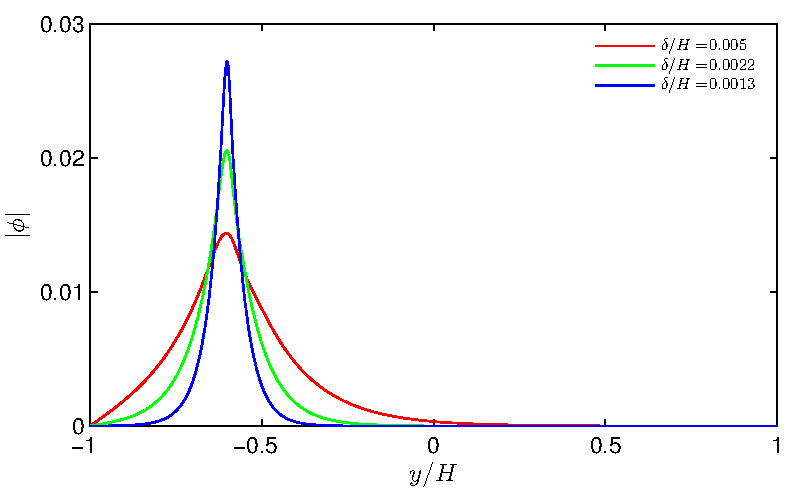
\includegraphics[scale=1.1]{Asymptotic_noshear}}\\
 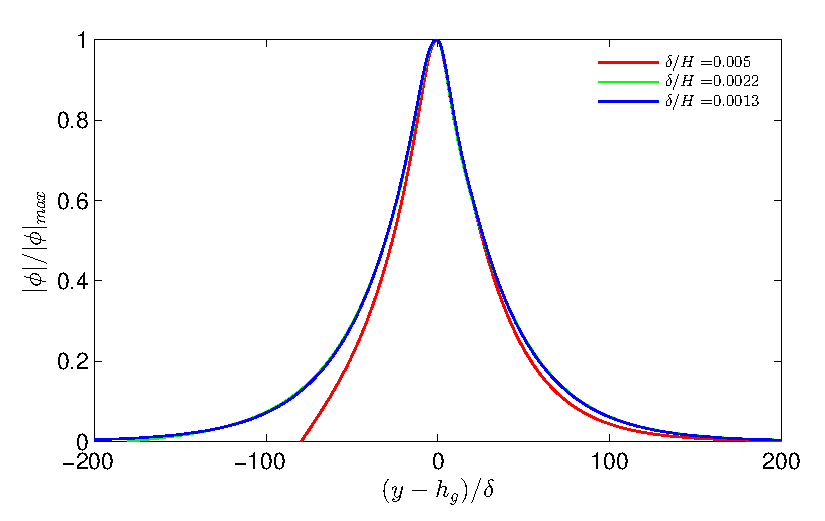
\includegraphics[scale=1.1]{Asymptotic_noshear2}
\caption[Plot of the neutral Mode 1 shape $|\phi|$ in the limit of small $\delta/H$ for $\hg/H=0.2$]{
Plot of the neutral Mode 1 shape $|\phi|$ in the limit of small $\delta/H$ for $\hg/H=0.2$ in the top panel.
% Mode 1 is shown in solid and Mode 2 is shown in dashed. The parameters for Mode 2 shapes are chosen such that $\Rey \gg 1$, $\Ndg \gg 1$ (specified in terms of $\delta/H$) but $\Rey/\Ndg = O(1)$. 
The approach of mode shapes to each other for these small values of $\delta/H$ indicates that the dense vegetation asymptote is reached. 
Mode 1 shapes appear self-similar in shape as $\delta\to 0$.
The bottom graphs shows rescaled $|\phi|$ for Mode 1 as a function of $(y-\hg)/\delta$ approach a universal shape, indicating that an asymptotic limit has been reached. 
% The limit is not yet reached for the case $\delta/H = 0.005$ due to the influence of bottom boundary; the vegetation height in this case is comparable to the boundary layer thickness.
}
\label{Asymptotic_mode}
\end{figure}

\subsection{Mode 2}
Our numerical observation for Mode 2 shows that threshold Reynolds number for Mode 2 scales as $\Rey \propto ({\delta}/{H})^{-3/2}$, which is shown in Figure \ref{Re_vs_delta}. The behavior of this critcal reynolds number can be understood by doing asymptotic analysis of equation \eqref{Orr-somerfield} in the limit $\Rey \gg 1$ and $\Ndg \gg 1$, we also observe that Mode 2 shows highest growth to a perturbation of $k \sim O(1)$ and the eigen value $\sigma$ is $O(1)$ as well. In the limit $\Rey \gg 1$ and $\Ndg \gg 1$, the non-dimensional flow in the grass bed is $U_g/U_0 \sim (\Rey \Ndg)^{-1/2} \ll 1$, and therefore $ikU \ll \sigma$, hence, $ikU$ may be neglected in comparison to $\sigma$. Furthermore, since $U(y)$ is approximately constant in the vegetation, $U_{yy}$ decays to zero within the grass outside the boundary layer. Using $D\sim 1$ and $U \sim 1$, outside the grass; the magnitude of advection term $\left(\sigma + i k U\right)\left(D^2- k^2\right) \phi$ is $O(1)$ and the 
magnitude of 
turbulent viscous stress term $(1/\Rey)\left(D^2-k^2\right)^2\phi$ is $O(1/R)$. In the limit $\Rey \gg 1$, the turbulent viscous term is negligible compared to the inertial term.
Thus, \eqref{Orr-somerfield} simplifies to 
\begin{subequations}
\begin{align}
% \begin{split}
\sigma\left(D^2-k^2\right)\phi = -2{(\Ndg/\Rey)^{1/2}}D^2\phi,  \quad &\text{ for } y<\hg  \label{eqn:mode2asympa} \\
\left(\sigma+ikU\right) \left(D^2-k^2\right)\phi =  ikU_{yy}\phi, \quad &\text{ for } y>\hg. \label{eqn:mode2asympb}
% \end{split}
\end{align}
\label{eqn:mode2asymp}
\end{subequations}
The above equation \eqref{eqn:mode2asymp} has only one parameter $\Rey/\Ndg$. 
So, for fixed $\Rey/\Ndg$, we expect that the mode shape converges in the aforementioned limit, which we can confirm from our numerical findings shown in Fig.~\ref{Asymptotic_mode2}. The convergence of mode shape in this limit indicates that we have identified the correct asymptotic limit to investigate Mode 2. We therefore expect that the  threshold is set by parameter $\Rey/\Ndg$, which can be further justified by the numerically observed asymptotic behavior $\Rey \propto \Ndg$ (or $\Rey \sim ({\delta}/{H})^{-3/2}$; see Fig.~\ref{Re_vs_delta} for comparison with numerical results).
The structure of this mode in the aforementioned limit is such that $\phi$ is continuous at $y=h_g$, but $D\phi$ undergoes a rapid transition on the scale of boundary layer thickness $\delta$ ( see figure \ref{Asymptotic_mode2}).
Furthermore, the eigenvalues and the mode shapes have very weak dependence on $\delta$. Since $u(x,y,t) =  D\phi e^{(ikx+\sigma t)}$, we conclude that the effect of rapid transition of the $D\phi$ on the scale of boundary layer near the grass tip have secondary role of regularizing the discontinuity in tangential velocity arising at $y=\hg$ in this instability mechanism.
The enhanced shear in the boundary layer plays no role for this mode of instability.
% We interpret Mode 2 as the instability of an inviscid fluid, with the vegetation modeled by a continuum drag field, and for which the boundary layer near the grass top plays no role. 
% On the other hand, Mode 1 asymptotically localizes to the boundary layer near the grass tip, and exhibits a different asymptotic behavior with $k \sim O(H/\delta)$, and $\Rey \sim (H/\delta)$ (or $\Rey \propto {\Ndg}^{1/2}$) at the threshold. 
\begin{figure}
\centerline{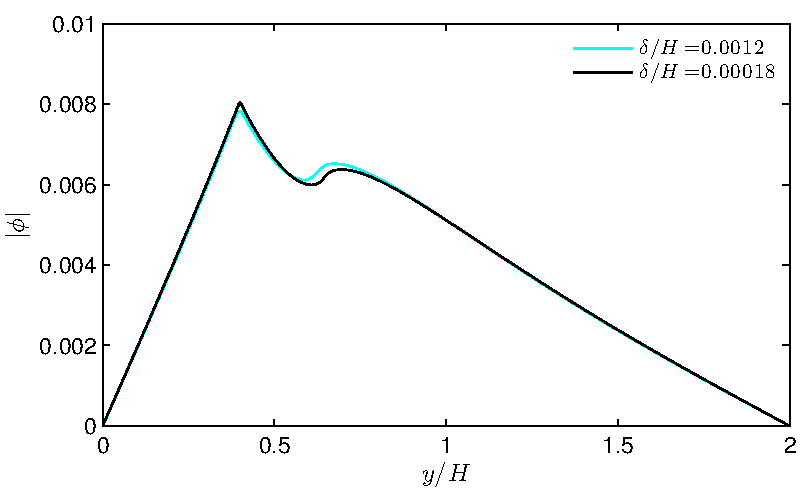
\includegraphics[width=1\linewidth]{AsymptoticPhiNoshear}}
\centerline{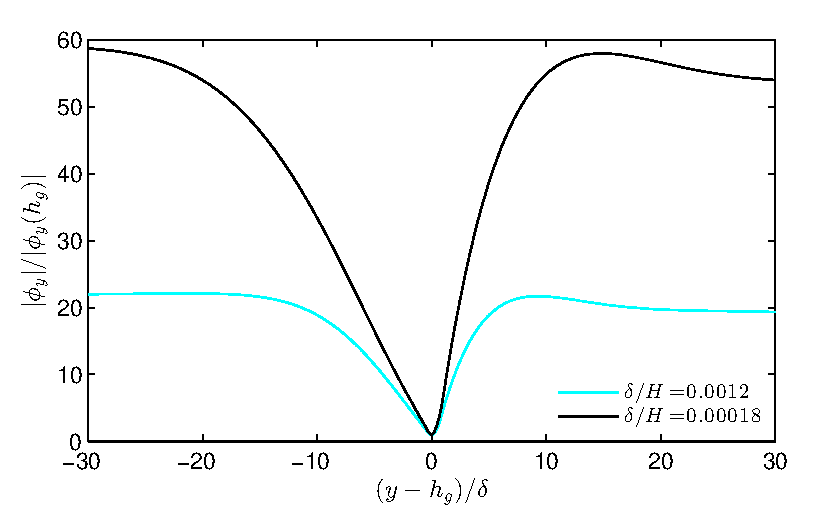
\includegraphics[width=0.95\linewidth]{AsymptoticPhiyNoshear}}
\caption[Plot of the neutral Mode 2 shape $|\phi|$ in the limit of small $\delta/H$ for $\hg/H=0.2$]{
Plot of the neutral Mode 2 shape $|\phi|$ in the limit of small $\delta/H$ for $\hg/H=0.2$ in the top panel.
The approach of mode shapes to each other for these small values of $\delta/H$ indicates that the dense vegetation asymptote is reached. 
The bottom graphs shows that $\phi_y$ undergoes rapid transition on the scale of boundary layer thickness $\delta$.
}
\label{Asymptotic_mode2}
\end{figure}

The dependence of Mode 2 on the perturbation of wavenumber $k$ (see Figure \ref{K_Re_sigma_set3}) and the structure of mode (see Figure \ref{Asymptotic_mode2}) suggest that Mode 2 has characteristics distinct from KH. We can also understand the difference between Mode 2 and the KH instability by observing that outside the grass, the unstable mode shape is governed by the inviscid Rayleigh's equation \eqref{eqn:Rayleigh}.
According to Rayleigh's criteria \cite{Rayleigh1879}, an inflection point in $U(y)$ is a necessary condition for instability arising from \eqref{eqn:Rayleigh}. However, with the current model $U_{yy}(y) = -1$ above the grass and therefore does not change sign for $y>\hg$. 
Instead, the dynamics are coupled with the flow in the grass bed described by \eqref{eqn:mode2asympa} in $y< \hg$.
The absence of $U_{yy}$ in \eqref{eqn:mode2asympa} indicates that $U_{yy}$ is approximated to be zero in $y<\hg$, and therefore the positive values of $U_{yy}$ that occurs in the boundary layer do not affect this mode of instability to the leading order.
Therefore, we conclude that Mode 2 is distinct from the KH instability as well, and owes its existence to the vegetation drag.
% \subsection{Comparison with KH}
% Table \ref{tab:comparison} compares the two modes to each other, and to the KH instability. 
% Because the eigenfunction of Mode 1 is localized over a length scale $\delta$, it may be interpreted as the instability of the flow in the boundary layer, whereas Mode 2 may be  % understood as the instability on the scale of the water column. 
% Mode 1 appears to be superficially similar to the Kelvin Helmholtz mechanism, whereas Mode 2 arises purely from the interaction between the unvegetated water column and the flow through the vegetation. 
% The appearance of the vegetation drag parameter in the dominant balances represented by ~\eqref{eqn:mode1asymp} and ~\eqref{eqn:mode2asymp}, and the resulting threshold criteria % demonstrates its role in setting the threshold, and in distinguishing them from the KH instability.
% Vegetation drag plays a dominant role in the mechanism for both the modes, which distinguishes our analysis from the traditional KH instability. 

%\lipsum[101-120]

\begin{table*}
% \footnotesize
\rowcolors{3}{tableShade}{white}  %% start alternating shades from 3rd row
\renewcommand{\arraystretch}{1.2}
 \begin{tabular}{l|c|c|c}
			& KH 				& Mode 1 		& Mode 2 \\ \hline
 Base velocity profile 	& $U(y) = U_0 \tanh(y/\delta)$			& \multicolumn{2}{c}{Equation \eqref{base_equ}} \\
 Domain 		& $-\infty < y < \infty$			& \multicolumn{2}{c}{$-1<y<1$} \\
 Inflection point	& exists at $y=0$				& \multicolumn{2}{c}{$U''(y)$ discontinuous at $y=\hg$} \\
 Shear layer thickness	& $\delta$					& \multicolumn{2}{c}{$\delta \sim  H\left(\Rey \Ndg \right)^{-1/3}$} \\
 Linearized dynamics	& Equation \eqref{eqn:Rayleigh}		& \multicolumn{2}{c}{Equation \eqref{Orr-somerfield}} \\
 Dense grass limit &  no grass included & Equation \eqref{eqn:mode1asymp} & Equation \eqref{eqn:mode2asymp}  \\
 Critical parameters	& none						& $\Rey \propto \Ndg^{2}$ 	& $\Rey \propto \Ndg$ \\
 Most unstable $k$ as $\delta \to 0$	& $\propto H/\delta$		& $\propto H/\delta$	& $O(1)$ \\
 Mode localized?	& yes, near $y=0$				& yes, near $y=\hg$			& no, spans water column
 \end{tabular}
 \caption{Comparison between KH instability and the two unstable modes resulting from solution of \ref{Orr-somerfield}.}
 \label{tab:comparison}
\end{table*}
\clearpage{\pagestyle{empty}\cleardoublepage}

\subsection{Comparison with the experimental data}
\begin{figure}
\centerline{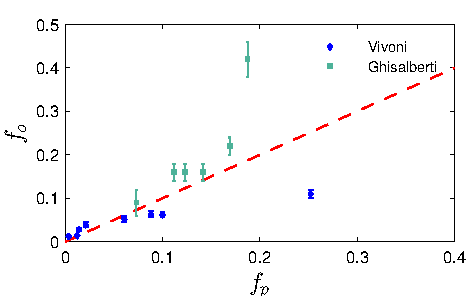
\includegraphics[]{new_graph_freq}}
\caption[Comparison of the experimentally measured dominant frequency $f_o$ (in Hz) with the predictions $f_p=\text{Im}(\sigma)$ from the solution of equation ~\eqref{Orr-somerfield}]{Comparison of the experimentally measured dominant frequency $f_o$ (in Hz) with the predictions $f_p=\text{Im}(\sigma)$ from the solution of equation ~\eqref{Orr-somerfield}. 
The experimental data in the inset is obtained from \cite{Ghisal02} (Ghisalberti) and \cite{Vivoni98} (Vivoni). 
In order to estimate the $\Rey$ for these experiments, a representative value of $\mu=0.1$ Pa~s was assumed.
}
\label{frequency_comparison}
\end{figure}
We have compared the prediction of critical Reynolds number with the data observed in the lab scale experiments. It is found to compare well \cite{Ghisal02} (see Figure \ref{Re_vs_delta}). The frequency (Im$(\sigma)$/2$\pi$) of the fastest growing mode also agrees well with observed frequency of {\monami} which is estimated from maxima in the velocity spectra, and frequency of vortex passage in lab scale experiments \cite{Ghisal02}, for cases where the vegetation was sufficiently dense to be modeled by a continuum drag field as shown in Fig.~\ref{frequency_comparison}. The comparison of solution of \eqref{base_equ}
with the experimentally measured velocity profile in the lab scale experiment of Vivoni \cite{Vivoni98} are shown in ~\ref{VivoniFig}. The velocity profile for experiment of Ghisalberti \cite{Ghisal02} are not available for comparison. The calculated velocity profiles for these experiments are estimated using the constraint of given flow rate, grass number density and the submergence ratio. We have used a constant representative value of eddy viscosity $\mu =  \text{0.1 Pa s}$. We observe that there are large variation between the experimentally measured frequency of Ikeda \cite{Ikeda96} and the  frequency predicted by the solution of \ref{Orr-somerfield}, the reason for this disagreement might be applicability of the current model to the experimental set up of Ikeda \cite{Ikeda96}, which can be seen from the comparison between the experimentally measured velocity and the velocities estimated from the solution of \eqref{base_equ} (see Figure \ref{IkedaMatching}). We see that for the case of Ikeda \cite{
Ikeda96}, the boundary 
condition at the 
bottom of the grass can not be approximated by zero shear, hence we do not expect the prediction of current model to agree well with the experimental data of Ikeda \cite{Ikeda96}.

Although the experimentally observed \monami ~wavelengths are not available for comparison, the predicted wavelength for lab scale experiments \citep{Ghisal02} are found to be $O(H)$.
\begin{figure}
 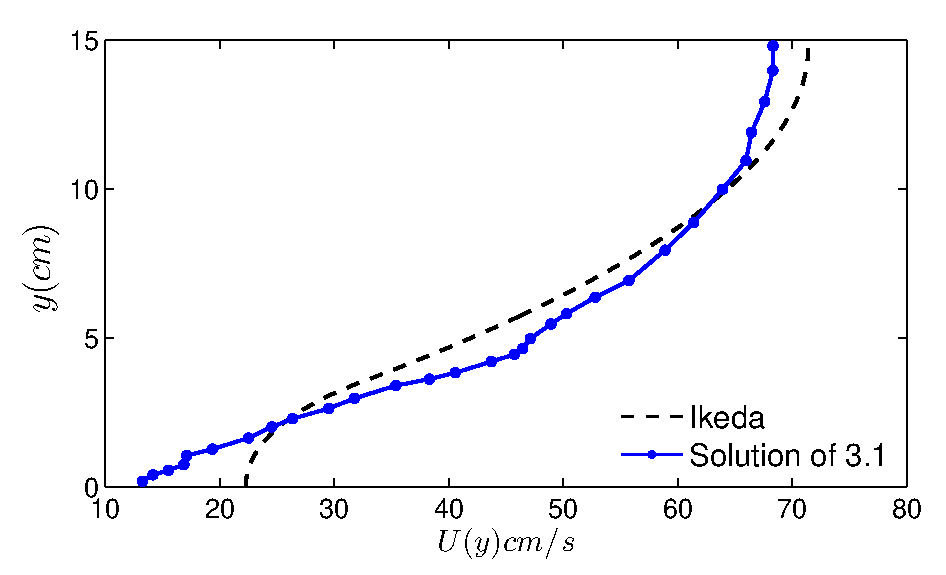
\includegraphics{Ikeda_zero_shear_match}
 \caption[ Comparison of experimental velocity profile of lab scale experiments with the solution of equation \eqref{base_equ} for \textit{Run 1 } experimental observation of Ikeda \cite{Ikeda96}. ] { Comparison of experimental velocity profile of lab scale experiments with the solution of equation \eqref{base_equ} for \textit{Run 1 } experimental observation of Ikeda \cite{Ikeda96}. The graph with solid line represents experimental data and the dashed line represent the estimated velocity profile from the solution of \eqref{base_equ}.    }
 \label{IkedaMatching}
\end{figure}

\begin{figure}
 {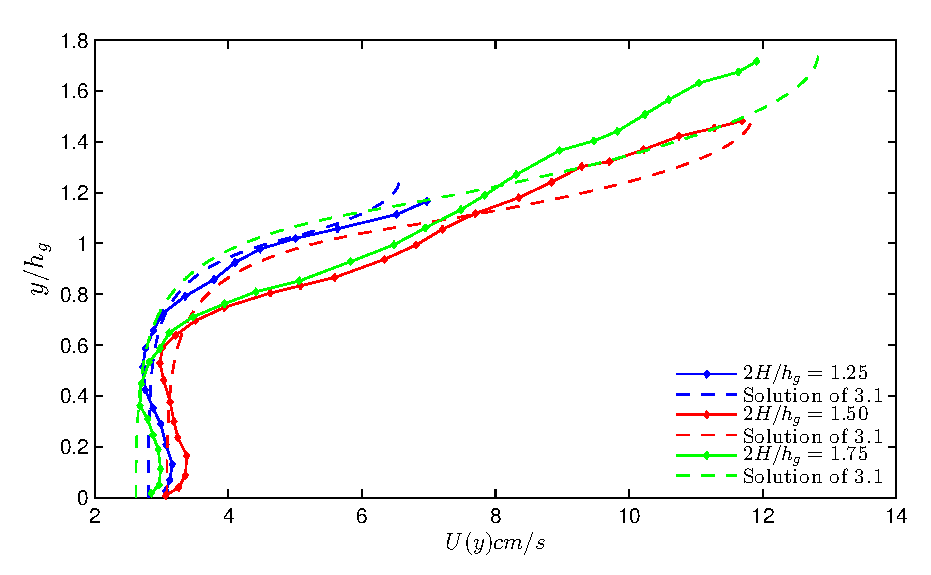
\includegraphics[]{Vivoni_Fig3_6_zero_shear_match}\\
 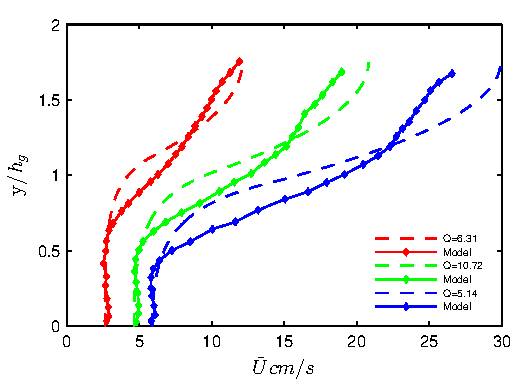
\includegraphics{Vivoni_Fig3_7_zero_shear_match}}
 \caption[ Comparison of experimental velocity profile of lab scale experiments with the solution of \eqref{base_equ} for \textit{Case A } and \textit{Case B} on experimental observation of Vivoni \cite{Vivoni98}.]{Comparison of experimental velocity profile of lab scale experiments with the solution of \eqref{base_equ} for \textit{Case A } (on top) and \textit{Case B} on (bottom ) experimental observation of Vivoni \cite{Vivoni98}. The graph with solid line represents experimental data and the dashed line with same color represent the estimated velocity profile from the solution of \eqref{base_equ}.  }
 \label{VivoniFig}
\end{figure}


\chapter{Nonlinear Solution of flow through submerged grass}
\section{Numerical Method}
We explicitly solved equation
\eqref{averaged_eq} with a finite difference method on a staggered grid using a {\bf{MAC}} (marker and cell) scheme, subject to periodic boundary condition in $x$. On this staggered grid, pressure variables are defined at the center of the cell, the x-component of velocity $u$ is defined on the center of vertical faces and the vertical velocity $v$ is defined on the center of horizontal faces, as shown in the Figure \ref{staggered}.
In this method, each time step is divided into two substeps. In the first step we ignore pressure and solve convection and diffusion equation,
\begin{figure}
\centerline{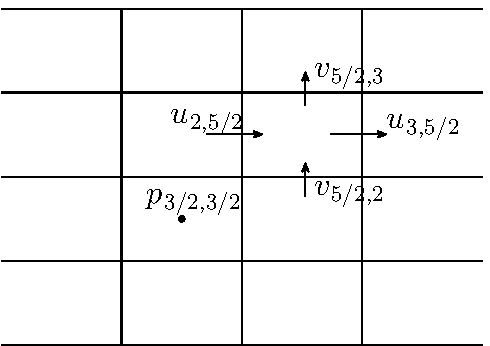
\includegraphics{StaggardGrid}}
\caption[Staggered grid showing the grid points of $u$, $v$ and $p$ field.]{Staggered grid showing the grid points of $u$, $v$ and $p$ field. The horizontal velocity $u$ is defined at the center of vertical faces of the cell, vertical velocity $v$ is defined at the center of horizontal faces and the pressure is defined at the center of the cell.   }
\label{staggered}
\end{figure}
\begin{equation}
\frac{\tilde{\bu}^{n+1}-\bu^{n}}{\Delta t}+(\bu^n \cdot \grad )\bu^n - \frac{1}{R} \grad^2 \bu^n -\Ndg (u^2)^n\bx,
\label{TransportEq}
\end{equation}
where $\Delta t$ is the size of time discretization, n denotes time label and $R$ is the Reynolds number. In the second step, we add pressure gradient operator and impose the incompressibility of flow.
\begin{equation}
\begin{split}
 \frac{\bu^{n+1}-\tilde{\bu^{n+1}}}{\Delta t} +\grad P^{n+1} &= 0\\
 \grad \cdot \bu^{n+1} = 0
 \label{IncompressibleCondEq}
 \end{split}
\end{equation}
Using the staggered grid the two components of equation \eqref{TransportEq} can be written as
\begin{equation}
\begin{split}
 \tilde{u}_{i,j+1/2}^{n+1} &= u_{i,j+1/2}^n - \Delta t \left(u u_x + vu_y -\frac{1}{R}\grad^2u \right)_{i,j+1/2}^n -\Delta t\Ndg (u^2)_{i,j+1/2}^n\\
 \tilde{v}_{i+1/2,j}^{n+1} &= v_{i+1/2,j}^n - \Delta t \left(u v_x + vv_y -\frac{1}{R}\grad^2v \right)_{i,j+1/2}^n
\end{split}
\end{equation}
where $\left(u u_x + vu_y -\frac{1}{R}\grad^2u \right)_{i,j+1/2}^n$ and $\left(u v_x + vv_y -\frac{1}{R}\grad^2v \right)_{i,j+1/2}^n$
needs to be evaluated at the grid location for the x-component of velocity at $(i,j+1/2)$ and for y-component of the velocity at $(i+1/2,j)$, respectively. The equations \eqref{IncompressibleCondEq} are discretized as 
\begin{equation}
\begin{split}
 u^{n+1}_{i,j+1/2} &= \tilde{u}^{n+1}_{i,j+1/2} -\frac{1}{R} \frac{\Delta t}{\Delta x} \left(p_{i+1/2,j+1/2}^{n+1} -p_{i-1/2,j+1/2}^{n+1} \right)\\
 v^{n+1}_{i+1/2,j} &= \tilde{v}^{n+1}_{i+1/2,j} -\frac{1}{R} \frac{\Delta t}{\Delta y} \left(p_{i+1/2,j+1/2}^{n+1} -p_{i+1/2,j-1/2}^{n+1} \right)
 \end{split}
 \label{true_velocity_cmp}
\end{equation}
where $\Delta x$ and $\Delta y$ are the uniform grid spacing in the x and y directions, respectively. The continuity equation on this staggered can be written as 
\begin{equation}
 \frac{ u_{i+1,j+1/2}^{n+1}-u_{i,j+1/2}^{n+1} }{ \Delta x } +\frac{v_{i+1/2,j+1}^{n+1}-v_{i+1/2,j}^{n+1} }{\Delta y} = 0
 \label{staggered_continuity}
 \end{equation}
Substituting the velocity components from equation \eqref{true_velocity_cmp} into equation \eqref{staggered_continuity}, we get discretized poisson equation for pressure.
\begin{equation}
\begin{split}
  \Delta t \left[\frac{p_{i+3/2,j+1/2}^{n+1}-2p_{i+1/2,j+1/2}^{n+1}+p_{i-1/2,j+1/2}^{n+1}}{\Delta x^2} \right] &+
 \Delta t \left[ \frac{p_{i+1/2,j+3/2}^{n+1}-2p_{i+1/2,j+1/2}^{n+1}+p_{i+1/2,j-1/2}^{n+1}}{\Delta y^2}   \right] = \\
 \frac{\left(\tilde{u}_{i+1,j+1/2}^{n+1}-
  \tilde{u}_{i,j+1/2}^{n+1}  \right) }{\Delta x}&+\frac{\left(\tilde{v}_{i+1/2,j+1}^{n+1}-\tilde{v}_{i+1/2,j}^{n+1}  \right)}{\Delta y}
\end{split}
\label{pressure_equation}
\end{equation}
The zero normal velocity on the top and bottom surface provides the boundary condition for pressure field, which are used to solve for pressure using \eqref{pressure_equation}. Substituting the pressure from the solution of equation \eqref{pressure_equation} into equation \eqref{true_velocity_cmp} we get the velocity field at the next time step. 
\begin{figure}
\centerline{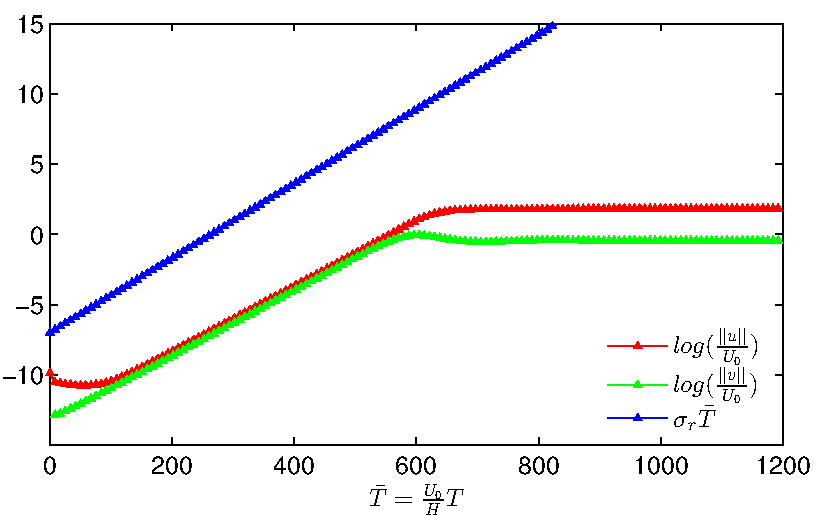
\includegraphics{LinearStabilityVsCFD1} }
\caption [Graph showing growth rate of a random perturbation made to the solution of \eqref{base_equ}, by explicitly solving \eqref{averaged_eq} and its comparison with the highest growth rate predicted by linear stability analysis.  ] {Graph showing growth rate of a random perturbation made to the solution of \eqref{base_equ}, by explicitly solving \eqref{averaged_eq} and its comparison with the highest growth rate predicted by linear stability analysis. The $\sigma_r$ is the real part of growth rate predicted by linear stability analysis. The  Reynolds number, grass number density and submergence ratios are $R=250$, $\Ndg=2$ and $h_{g}/(2H) = 0.4$ respectively.}
\label{CFD_vs_LinearStabilityGrowthRate}
\end{figure}
\section{Comparison with linear stability analysis}
We have explicitly solved equation \eqref{averaged_eq} with the initial condition $u(x,y,0) = U_{0}(y)+\tilde{u}_0(y)$ and $v(x,y,0)=0$, where $U_{0}(y)$ is velocity profile arising from the solution of equation \eqref{basicflow} and $\tilde{u}(y) = \epsilon f(y)$ is a random perturbation to $U_0(y)$, where $\epsilon \ll 1$ and $f(y)$ is an arbitrary function. We expect this perturbation to grow exponentially as $||u(t)|| = ||u(t_0)|| e^{\sigma_r (t-t_0)}$ with the maximum growth rate ($\sigma_r$) as predicted by the solution of equation \eqref{Orr-somerfield}, where $||.||$ represents $L_2$ norm of perturbation. A comparison of growth rate computed from the solution of equation \eqref{averaged_eq} with the
maximum growth rate $\sigma_r$ predicted from the solution of equation \eqref{Orr-somerfield} is shown in Figure \ref{CFD_vs_LinearStabilityGrowthRate}. We can see that initially when the perturbation to the $U_0(y)$ is small, the perturbation grow with the rate predicted by equation \eqref{Orr-somerfield}. However, once the magnitude of perturbation becomes comparable to the $U_0(y)$, non-linear effect also becomes important and the growth rate can not be described by the solution of linear stability analysis. 

In the regime when $||u-U_0|| \ll ||U_0||$, we also expect that the profiles of perturbation velocities $\tilde{u}(x,y,t) = u(x,y,t) - U_0(y)$ and $\tilde{v}(x,y,t) = v(x,y,t)$ can be easily described by the dominant eigen mode $\phi(k,y)$ corresponding to $k$ with the highest growth rate
\begin{equation}
\begin{split}
 \tilde{u}(x,y,t) &= \Re\left(\phi_y(k,y) e^{ikx+\sigma t+ i\theta}\right),\\
 \tilde{v}(x,y,t) &= \Re\left(ik \phi(k,y) e^{ikx+\sigma t + i\theta }\right).
\end{split}
\end{equation}
Where $\theta$ is a constant phase between $\tilde{u}(0,y,t)$ and $\Re(\phi_y(k,y) e^{\sigma t})$. A comparison between initial evolution of perturbation variables $(\tilde{u}, \tilde{v}, \tilde{p})$ with a random perturbation to the base flow $U_0(y)$ arising from the solution of equation \eqref{averaged_eq} with the prediction based  on the dominant eigen-mode $\phi(k,y)$ is shown in Figure \ref{CFD_vs_LinearStability_AllVariables}; which shows expected agreement between prediction based on the dominant eigen mode analysis and the prediction based on the full numerical simulation of equation \eqref{averaged_eq}.

By carrying out numerical simulation of equation \eqref{averaged_eq} for large time, we observe that initially the amplitude of perturbation variable grow with the rate predicted by linear stability analysis and then saturates to constant value (  See Figure \ref{CFD_vs_LinearStabilityGrowthRate} ). After the perturbation saturates to an approximately constant value, the flow can be described as a steadily propagating wave (see figure \ref{VorticityColor} ). The frequency and wavelength of the wave arising from the flow instability can be easily calculated by observing the vortex passage frequency near the grass tip and the vortex pattern over the flow domain (see figure \ref{TimeVsVorticity} and figure \ref{XVsVorticity} ). If the Reynolds number is close to the critical value, we expect the frequency and wavelength of the wave arising due to flow instability to be comparable to the one predicted by linear stability analysis. A comparison between prediction of wavelength and frequency based on the solution 
of equation \eqref{Orr-somerfield} and equation \eqref{averaged_eq} is shown in table \ref{tab:LinearStabilityVsCFD}. In figure \ref{CFDVsLinearStabilitySaturated}, we have also shown comparison between $u(x,y,t)- \langle u(y,t) \rangle$ and 
 $\Re\left(\phi_y(k,y) e^{i\left(kx+\sigma_i t+ \theta\right)} g(t) \right)$  and between $v(x,y,t)-\langle v(y,t) \rangle$ and $\Re\left(\phi(k,y) e^{i\left(kx+\sigma_i t+ \theta\right)} g(t) \right)$, for Reynolds number close to its critical value. Where $u(x,y,t)$ and $v(x,y,t)$ are solution of equation \eqref{averaged_eq}, $\sigma_i$ is the imaginary part of the eigenvalue predicted by the solution of equation \eqref{Orr-somerfield} corresponding to the maximum growth rate $(\Re(\sigma))$, $\phi(k,y)$ and $\phi_y(k,y)$ are the dominant eigen mode and it's derivative corresponding to $k$ with the highest growth rate, $g(t)$ is amplitude of $u$ and $v$ and $\langle  \rangle$ denotes horizontally averaged variables, i.e.,
 \[\langle u(y,t) \rangle = \frac{1}{L}\int_{0}^{L} u(x,y,t) dx .\]
 Similar comparison for pressure is also shown in figure \ref{CFDVsLinearStabilitySaturated}. From the agreement between the explicit numerical calculation and the prediction based on the solution of Orr-Sommerfeld equation \eqref{Orr-somerfield}, we can infer that for Reynolds number $R$ close to it's critical value, the flow in the saturation region ( for $T(U_0/H)>600$ ) can be described as steadily propagating wave whose wavelength, frequency and mode shape is close to that predicted by linear stability analysis.  
\begin{centering} 
\begin{table}
\begin{tabular}{|c|c|c|c|c|}
\hline
  Reynolds Number 
   &\multicolumn{2}{c|}{Linear Stability Analysis }&\multicolumn{2}{c|}{ Solution of \eqref{averaged_eq}}\\
\cline{2-5}
 & $H k$
 & $\omega (H/U_0)$ & $ H k$  &  $\omega (H/U_0)$ \\
\hline
$ R = 250 $ &    1.35 & 0.535 & 1.256 &  0.505 \\
$ R = 300 $ &    1.50 & 0.567 & 1.256 &  0.468 \\
$ R = 400 $ &    1.50 & 0.541 & 1.256 &  0.386 \\
$ R = 500 $ &	  1.50 & 0.523 & 1.256 &  0.325 \\
$ R = 600 $ &	  1.50 & 0.509 & 1.570 &  0.363 \\
$ R = 700 $ &     1.65 & 0.538 & 1.570 &  0.311 \\

\hline
\end{tabular}
 \caption{Comparison between the estimates of frequency and wavelength between prediction based on the solution of \eqref{Orr-somerfield} and \eqref{averaged_eq}. The calculation is done for $\Ndg=2$, $h_g/(2H)=0.4$. The critical Reynolds number is $R=190$ .}
 \label{tab:LinearStabilityVsCFD}
\end{table}
\end{centering}

\begin{figure}
\centerline{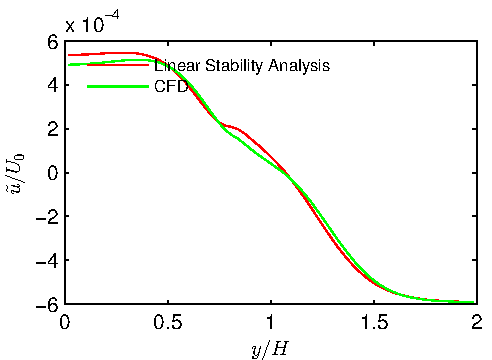
\includegraphics{LinearStabilityVsCFD_u_phase0} 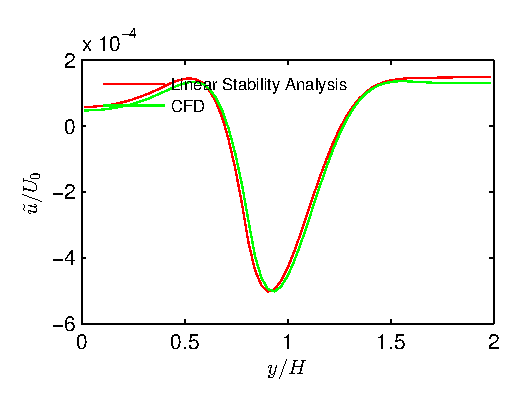
\includegraphics{LinearStabilityVsCFD_u_phase90}}
\centerline{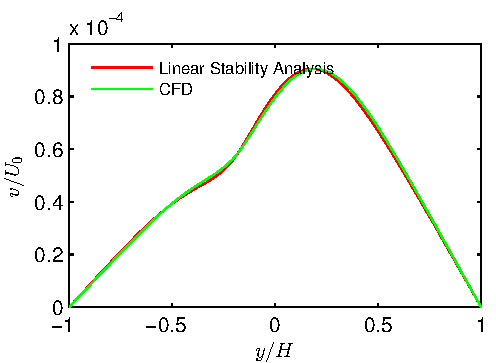
\includegraphics{LinearStabilityVsCFD_v_phase0} 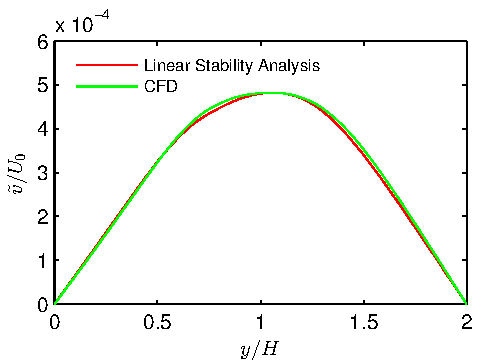
\includegraphics{LinearStabilityVsCFD_v_phase90}}
\centerline{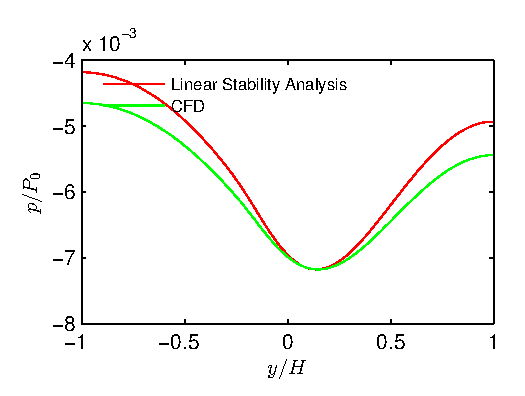
\includegraphics{LinearStabilityVsCFD_p_phase0} 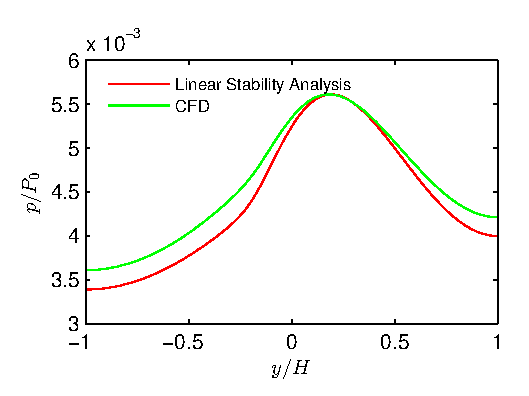
\includegraphics{LinearStabilityVsCFD_p_phase90}}
\caption [Comparison of velocities and pressure predicted by Linear Stability analysis and by explicitly solving equation \eqref{averaged_eq}. ]{Comparison of velocities and pressure predicted by Linear Stability analysis and by explicitly solving equation \eqref{averaged_eq}. The comparison are made at $\bar{T}=360$ and two different locations, where velocities are $\pi/2$ out of phase with each other. The parameters used are $R=250$, $\Ndg=2$, $h_g/(2H)=0.4$   .}
\label{CFD_vs_LinearStability_AllVariables}
\end{figure}
\clearpage{\pagestyle{empty}\cleardoublepage}

%\section{Saturated Region}
\begin{figure}
 \centerline{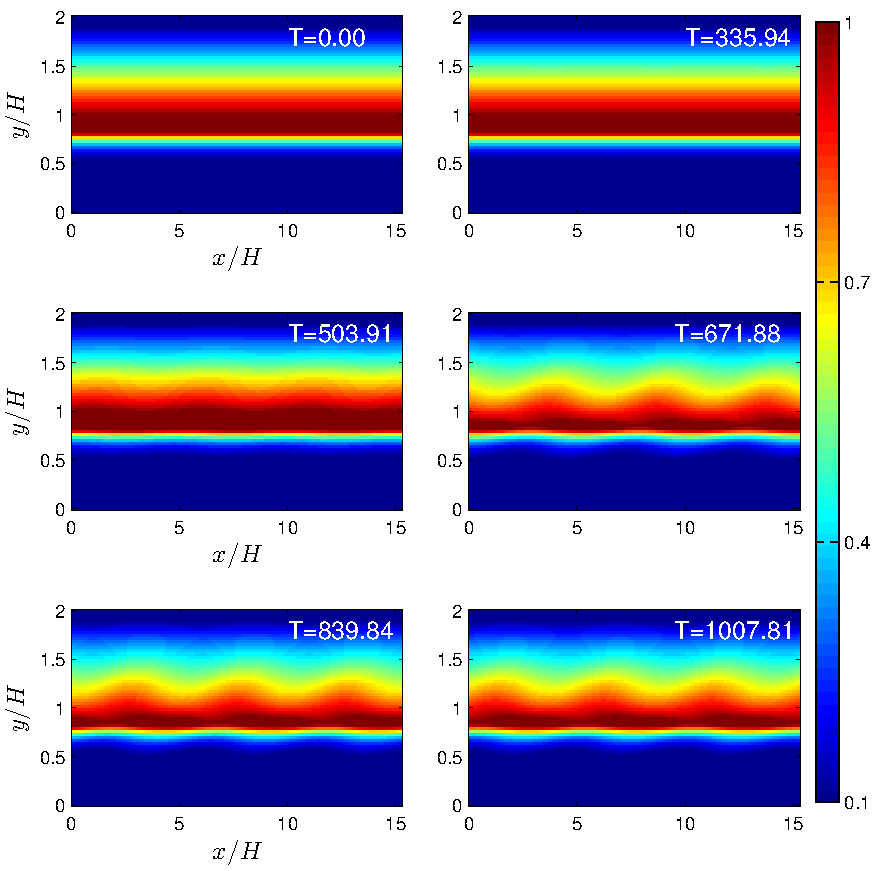
\includegraphics[scale=1.3]{VorticityColor}}
 \caption [ evolution of vorticity $\omega = \grad \times \bu$ as function of time for a random perturbation over the steady flow arising from the solution of \eqref{base_equ}. ]{ evolution of vorticity $\omega = \grad \times \bu$ as function of time for a random perturbation over the steady flow arising from the solution of \eqref{base_equ}. The perturbation grow with the rate predicted by linear stability analysis for $T(U_0/H)<400$ and then saturates to an approximately constant value. For $T(U_0/H) >400$ flow can be described as a steadily propagating wave, whose wavelength and frequency matches with the one predicted by linear stability analysis. The simulation is done for $R=250$, $\Ndg=2$ and $h_g/(2H)=0.4$ . } 
\label{VorticityColor}
\end{figure}

\begin{figure*}
\centerline{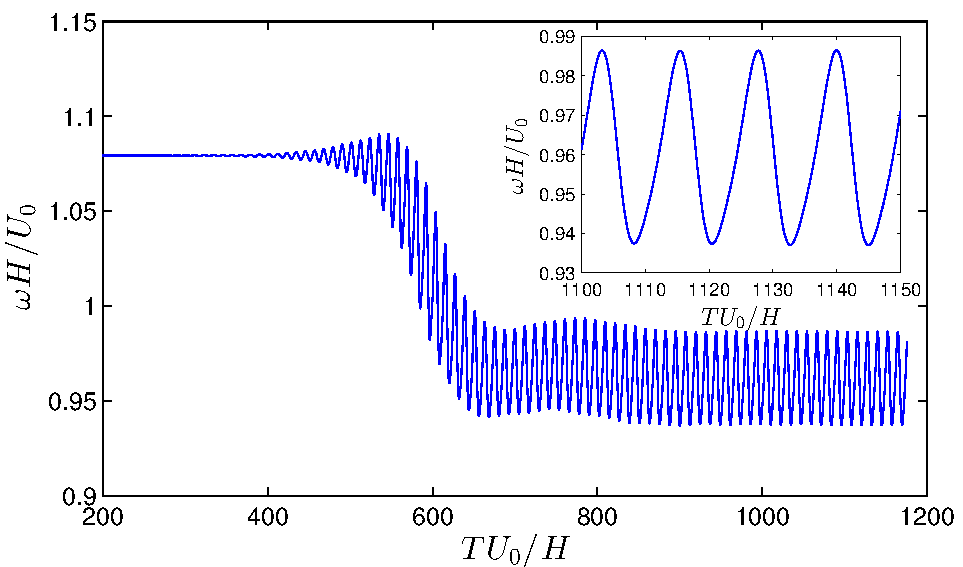
\includegraphics[scale=0.95]{LinearStabilityVsCFD_TimeVsVorticity}}
\caption[Plot of vorticity at the grass tip as function of time. ]{Plot of vorticity at the grass tip as function of time, from this plot we can estimate frequency of vortex passage at any time, the calculated frequency matches with the imaginary part of eigen value arising from the solution of equation \eqref{Orr-somerfield} corresponding to $k$ with the highest growth rate. The parameter used in this simulation is $R=250$, $\Ndg=2$, $h_g/(2H)=0.4$ .}
\label{TimeVsVorticity}
\end{figure*}

\begin{figure*}
\centerline{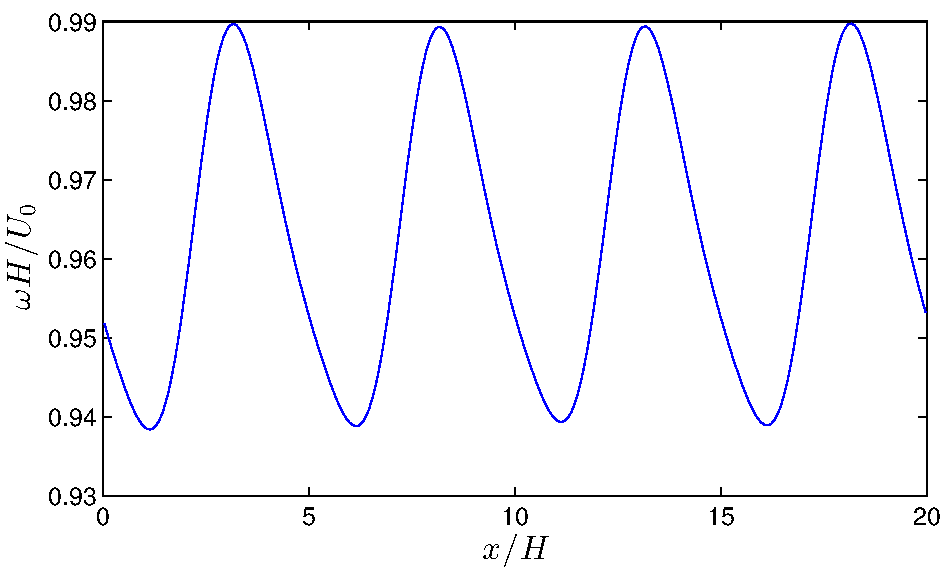
\includegraphics[scale=0.95]{LinearStabilityVsCFD_XVsVorticity}}
\caption [Plot of vorticity at the grass tip as function of x. ] {Plot of vorticity at the grass tip as function of x. The vorticity is calculated in the regime when the flow is saturated $T(U_0/H)=800$, from this plot we can estimate wavelength of vortex passage at the grass tip. The calculated wavelength  matches with wavenumber $k$ for which solution of equation \eqref{Orr-somerfield} predicts highest growth rate. The parameter used in this simulation is $R=250$, $\Ndg=2$, $h_g/(2H)=0.4$}
\label{XVsVorticity}
\end{figure*}

\begin{figure}
\centerline{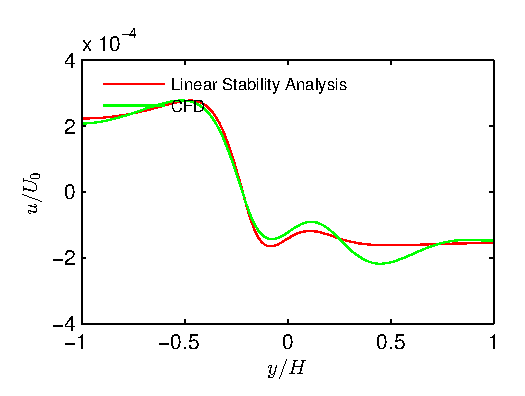
\includegraphics{LinearStabilityVsCFD_Saturated_u_phase0} \includegraphics{LinearStabilityVsCFD_Saturated_u_phase90}}
\centerline{\includegraphics{LinearStabilityVsCFD_Saturated_v_phase0} \includegraphics{LinearStabilityVsCFD_Saturated_v_phase90}}
\centerline{\includegraphics{LinearStabilityVsCFD_Saturated_p_phase0} \includegraphics{LinearStabilityVsCFD_Saturated_p_phase90}}
\caption [Comparison of velocities and pressure predicted by Linear Stability analysis and deviation of velocity and pressure from it's spatial average by explicitly solving equation \eqref{averaged_eq}. ] {Comparison of velocities and pressure predicted by Linear Stability analysis and deviation of velocity and pressure from it's spatial average by explicitly solving equation \eqref{averaged_eq}. The comparison are made at $\bar{T}=800$ and two different locations ($x/H=10$ and $x/H=35$ ), where velocities are $\pi/2$ out of phase with each other. The parameters used are $R=250$, $\Ndg=2$, $h_g/(2H)=0.4$ . }
\label{CFDVsLinearStabilitySaturated}
\end{figure}


\chapter{Linear stability analysis of flow around emergent vegetation}
\section{Introduction}
There are many situation in nature where there exists an interface between dense vegetation and a high conveyance channel, such as tidal creek with fringing mangroves, salt marshes and tidal channels etc. The difference of hydrodynamic drag between the vegetated plain and the main plain is characterized by strong shear in the velocity profile near the boundary of vegetated plain and the main channel, similar to the flow through submerged vegetation. Lab scale experiments simulating flow around emergent vegetation shows existence of coherent periodic vortices at the vegetation interface \cite{White07}. These coherent structures causes large momentum flux across the vegetation due to strong lateral motion which consists of sweeps toward vegetation and ejections away from the vegetation. The coherent structures also influence the exchange of mass and momentum between the two regions. The material exchange have been found to be of great importance for the hydrologic and ecological processes in the system. For 
example, the exchange of fresh water between a tidal creek and fringing mangrove is known to be extremely important in preventing hypersaline conditions which are harmful to the mangroves.  

\begin{figure}
\centerline{\includegraphics{GrassBaseIsotropicDrag}}
\caption [ Schematic diagram of conveyance channel adjacent to an emergent vegetation plain, and the schematic velocity profile in both regions. ] {Schematic diagram of conveyance channel adjacent to an emergent vegetation plain, and the schematic velocity profile in both regions. The green dot represents vegetation which comes out of the plane of the paper. The flow is directed in the x direction.}
\label{IsotropicSchematic}
\end{figure}
\section{Linear stability analysis}
The formation of coherent eddies near the vegetation interface under the influence of an otherwise steady current can be understood as result of some hydrodynamic instability. In order to understand the flow instability in the presence of flow around emergent vegetation, we perform a linear stability analysis of the system. In this analysis we use a continuum approximation of vegetation and represent the effect of vegetation as a continuum drag field. 
Since both component of flow $(u,v)$ in the vegetated region are across the vegetation, we approximate the effect of drag due to presence of vegetation by an isotropic drag field in the flow equation \eqref{averaged_eq}, which can be represented mathematically as,
\begin{equation}
 {\bf{D}} = -C|\bu|\bu.
 \label{IsotropicDrag}
\end{equation}
In order to perform linear stability analysis we first calculate fully developed steady solution $\bu = U(y) \bx$ of equation \eqref{averaged_eq} and equation \eqref{IsotropicDrag} driven by a constant pressure gradient $dP/dx$. Since the steady profile is in $x$ direction, the momentum balance equation \eqref{averaged_eq}
simplifies to the same from as equation \eqref{base_equ}, i.e.,
\begin{equation}
\begin{split}
 -&\frac{dP}{dx}+\mu U''(y) -S(y) \rho C d N_gU |U| =0,\\
 &S(y) = 1, \hspace{2cm} 0<y<\hg,\\
 &S(y) = 0, \hspace{2cm} \hg< y< 2H,
\label{Isotropicbase_equ}
\end{split}
\end{equation}
with the understanding that $h_g$ represents the extent of vegetation in the $y$ direction rather than vegetation height (see Figure \ref{IsotropicSchematic}). Since we are solving the same equation as equation \eqref{base_equ}, the base profile $U(y)$ from the solution of equation \eqref{Isotropicbase_equ} has the same structure as the one arising from the solution of equation \eqref{base_equ}. The base profile $U(y)$ is approximately uniform within vegetated region with 
$U(y) \approx U_g = \sqrt{\frac{-dP/dx}{\rho C d N_g}}$, and has parabolic velocity profile in the unvegetated region. The discontinuity of drag across the vegetation boundary along with the continuity of shear results in a boundary layer $\delta$ near the vegetation boundary. By performing analysis similar to the one done in section 3.1 we can derive the scaling of boundary layer $\delta \sim U_{bl}/U_0 \sim (R\Ndg)^{-1/3}$, where $U_{bl}$ is the scale of velocity in the boundary layer, $\mu$ is turbulent eddy viscosity, $U_0 = (-dP/dx)H^2/\mu$ is velocity scale in unvegetated region and $R = \rho U_0 H/\mu$ is the Reynolds number of the flow.
\subsection{Governing equation for flow instability}
We substitute $\bu = (U+\tilde{u}, \tilde{v})$, $p = (P+\tilde{p}) $ in ~\eqref{averaged_eq} and expand to linear order to investigate the evolution of small perturbations $(\tilde{u}, \tilde{v})$, which obey 
\begin{equation}
\begin{split}
\rho(u_t+U u_x+vU_y) &= -p_x+ {\mu}\nabla^2u-2S\rho C dN_{g}Uu, \\
\rho(v_t+ Uv_x) &= -p_y+ {\mu}\nabla^2v - S\rho C d N_g Uv, \hspace{0.3cm} \nabla\cdot\bu=0,
\label{LinearizedNavierStokesSymmetric}
\end{split} 
\end{equation}
we have drop tilde for convenience. Comparing \eqref{LinearizedNavierStokesSymmetric} with the \eqref{LinearizedNavierStokes}, we observe that the use of isotropic drag leads to an additional term in the $v$ momentum equation which lead to addition of an extra term in the equation  \ref{Orr-somerfield}, implying that to leading order the flow perturbation $(u,v)$ experiences additional drag for flow in vertical direction ($v$ component) as well due to $C d N_g Uv$ term in the $v$ component of the momentum equation. With stream function $\psi$ to satisfy mass balance and seeking a solution of the form $(u,v,\psi) = (\hat{u(y)},\hat{v(y)},\phi(y)) e^{ikx+\sigma t}$, we arrive at a modified form of Orr-Sommerfeld equation \cite{Drazin81,Chen97,Chu91}.
\begin{equation}
\begin{split}
\Rey^{-1}\left(D^2 -k^{2} \right)^2\phi = \left[ \left({\sigma}+ikU\right) \left(D^2-k^2\right) -ikU_{yy}\right]\phi + 
\Ndg D\left(2 S U D \phi\right) - \Ndg U k^2\phi,
\label{SymmetricOrr-somerfield}
\end{split}
\end{equation}
\subsection{Results}
Comparing equation \eqref{SymmetricOrr-somerfield} with \eqref{Orr-somerfield}, we notice that due to isotropic drag equation \eqref{SymmetricOrr-somerfield} have an additional dissipative term $ D_y = \Ndg U k^2 \phi$. %Through our numerical simulation we observe that one of the expected effect of this additional drag is to increase the stability of flow as compared to flow through vegetation due to presence of additional drag dissipation.
A heat map of $\Re (\sigma)$ as a function of $R$ and $k$ for different $h_g/H$ and $\Ndg$ is shown in figure \ref{Symmetric_Re_vs_delta}. The smallest $R$ on the neutral curve 
($\Re (\sigma)=0$) sets the threshold for flow instability. We observe that as $\Ndg$ increases, the unstable region splits into two. Similar to anisotropic drag case we refer to the region with higher $k$ as ``Mode 1'' and one with lower $k$ as ``Mode 2''; however the instability associated with large $k$ gets damped due to this additional drag dissipation and hence at large $\Ndg$, Mode 1 doesn't set the threshold for flow instability. The damping of Mode 1 at higher grass density can also be understood by observing that the additional drag $D_y \propto k^2$; hence, the flow instability associated with Mode 1 ( $k\propto H/\delta$ ) gets significantly damped compared to the instability associated with Mode 2 ($k\sim O(1)$). We numerically observe that threshold Reynolds number for large $\Ndg$ to be $ R \propto \Ndg$  or $R \propto (\delta/H)^{-3/2}$ ( see figure \ref{Symmetric_Re_vs_delta} ), similar to the case with anisotropic drag ( see figure \ref{Re_vs_delta} Mode 2 asymptote ). An analysis similar 
to one in section 4.3 can be done here as well to simplify the \ref{SymmetricOrr-somerfield}
\begin{subequations}
\begin{align}
% \begin{split}
\sigma\left( D^2-k^2\right)\phi = -2{(\Ndg/\Rey)^{1/2}}D^2\phi &+ (\Ndg/R)^{1/2} k^2 \phi,  \quad &\text{ for } y<\hg  \label{eqn:Symmetricmode2asympa} \\
\left(\sigma+ikU\right) \left(D^2-k^2\right)\phi =  ikU_{yy}\phi &, \quad &\text{ for } y>\hg. \label{eqn:Symmetricmode2asympb}
% \end{split}
\end{align}
\label{eqn:Symmetricmode2asymp}
\end{subequations}
The only remaining parameter in \eqref{eqn:Symmetricmode2asymp} is $\Rey/\Ndg$. The parameter $\Rey/\Ndg$ sets the threshold justifying the numerically observed asymptotic behavior $\Rey \propto \Ndg $ or $ \Rey \propto (\delta/H)^{-3/2}$. For fixed $\Rey/\Ndg$, the mode shape converges in the aforementioned limit, in agreement with the numerical result shown in figure \ref{IsotropicAsymptotic_mode}. The structure of mode in the aforementioned limit is such that $\phi$ is continuous at $y=h_g$, but $\phi_y$ undergoes a rapid transition on the scale of boundary layer thickness $\delta$ 
( see figure \ref{IsotropicAsymptotic_mode} ).

\begin{figure}
 \includegraphics{GrassBaseWhiteIsotropic}
 \caption [Comparison of steady profile from the solution of equation \eqref{Isotropicbase_equ} with that from the experiments in White \cite{White06} (Case X and Case I  ]{Comparison of steady profile from the solution of equation \eqref{Isotropicbase_equ} with that from the experiments in White \cite{White06} (Case X and Case I from figure 4.6 and figure 4.15) . }
 \label{GrassBaseWhiteIsotropic}
\end{figure}

A comparison of steady profile and the frequency of resultant flow instability with that of experimental observation of White in \cite{White06} is shown in Figure \ref{GrassBaseWhiteIsotropic} and in table \ref{tab:FrequencyComparisonIsotropicDrag}. The steady profile is calculated using the given flow rate constrain. Since these experimental data correspond to vegetation density for which both the mode have not split into two in the $R-k$ space ( see $\Ndg$ in \ref{tab:FrequencyComparisonIsotropicDrag} and column 1 in Figure \ref{IsotropicK_Re_sigma_set3}), we are unable to determine if the flow instability observed in the lab scale experiments are the result of Mode 1 instability or Mode 2 instability.
\begin{centering} 
\begin{table}
\begin{tabular}{|c|c|c|c|}
\hline
  Experimental details & Observed frequency & Calculated frequency & $\Ndg$ \\ 
\hline
 Case X &    0.112 & 0.068 &  3.5  \\
 Case I &    0.066 & 0.043 &  0.2 \\


\hline
\end{tabular}
 \caption{Comparison between the estimate of frequency with that from experimental observation of White in \cite{White06} (Case X and Case I from Figure 4.6 and Figure 4.15). The corresponding estimate of $\Ndg$ is also shown in the table. }
 \label{tab:FrequencyComparisonIsotropicDrag}
\end{table}
\end{centering}



\begin{figure}
 \centerline{\includegraphics{IsotropicAsymptoticNoshear}} 
 \centerline{\includegraphics{IsotropicAsymptoticPhiyNoshear}}
 \caption [ Plot of the neutral Mode 2 shape $|\phi|$ in the limit of small $\delta/H$ for $\hg/H=0.2$ ] {
Plot of the neutral Mode 2 shape $|\phi|$ in the limit of small $\delta/H$ for $\hg/H=0.2$ in the top panel.
The approach of mode shapes to each other for these small values of $\delta/H$ indicates that the dense vegetation asymptote is reached. 
The bottom graphs shows that $\phi_y$ undergoes rapid transition on the scale of boundary layer thickness $\delta$.
}
\label{IsotropicAsymptotic_mode}
\end{figure}
\begin{figure}
\centerline{ \includegraphics{IsotropicDragAll_imgsc4} }
\caption [ $\text{Re}(\sigma)$ and the neutral curve ($\text{Re}(\sigma)$=0) as a function of wavenumber and $\Rey$ for flow around emergent vegetation] {
$\text{Re}(\sigma)$ and the neutral curve ($\text{Re}(\sigma)$=0) as a function of wavenumber and $\Rey$ for parameters shown in the corresponding panel.  
As $\Ndg$ increases, the unstable region with higher $k$ value, i.e. the region corresponding to ``Mode 1'' become stable due to increase dissipation.
}
\label{IsotropicK_Re_sigma_set3}
\end{figure}

\begin{figure}
 \centerline{\includegraphics{IsotropicDragR_vs_delta}}
 \centerline{\includegraphics{IsotropicDragDeltaVsK}}
 \caption [Critical Reynolds number and the corresponding marginally stable wave number for different submergence ratio as a function of vegetation density  ] {
Critical Reynolds number ( top ) and the corresponding marginally stable wave number ( bottom ) for different submergence ratio as a function of vegetation density parametrized by the boundary layer thickness. }
\label{Symmetric_Re_vs_delta}

\end{figure}




\chapter{Discussion}
\section{Role of turbulence Model}
In our mathematical model we have used constant eddy viscosity, with this simple assumption about eddy viscosity, we are able to capture essential features of the flow instability. However, in a real flow the eddy viscosity varies with position, so this simple assumption about constant eddy viscosity only provide qualitatively accurate description of flow. 
%of We have modeled turbulence using a constant eddy viscosity. 
%The simplicity of this model allows us to make progress and capture the essential features of the instability. 
% without accounting for the rich and detailed characteristics of the turbulence. 
%However, this simplicity in some cases only provides a qualitatively accurate description of the flow. 
In this chapter, we present an account of the advantages and shortcomings of assuming a constant eddy viscosity to model the turbulence.

One of the consequence of using constant eddy viscosity is that the boundary layer thickness $\delta$ scales as $H(\ReyNdg)^{-1/3}$; however,
lab scale experimental observations carried by Nepf \cite{Nepf07} show that the boundary layer thickness scales instead as $\Ndg^{-1}$ \cite{Nepf07}.
Since the scaling of boundary layer arrive due to balance of viscous stress and drag force in the boundary layer, the precise nature of scaling is dependent on the precise nature of eddy viscosity used in the model. While the precise scaling of boundary layer thickness is governed by the details of the turbulence model, the existence of this boundary layer for dense vegetation is independent of the turbulence model. In this analysis we have captured one possible realization of this feature using constant eddy viscosity.
Experiments have also shown that a model based on constant mixing length $l$ better approximates the turbulent characteristics of the flow with $l \sim \delta$ \cite{White06,Nepf07}; \textit{i.e.}, assuming that the boundary layer itself establishes eddies to transport momentum. 
The eddy viscosity corresponding to this model can be approximated as $\mu \sim \rho U \delta$, and the dominant balance between turbulent momentum transport and vegetation drag in the boundary layer is  $\mu U/\delta^2 \sim \rho C_N d N_g U^2$.
Substituting $\mu$ and solving for $\delta$ yields $\delta/H \sim \Ndg^{-1}$, which is in agreement with the experimental observations.

% Replacing the constant eddy viscosity by the scale for it from the mixing length hypothesis also recovers the experimentally observed scaling for boundary layer thickness.
The scaling of experimentally observed boundary layer thickness $\delta \propto \Ndg^{-1}$ can also be understood with in the framework of our model. 
The mixing length model implies that near the grass tip, eddy viscosity scales as $\mu \sim \rho \ubl \delta$, which in turn corresponds to an effective $\Rey \sim U_0H/\ubl \delta$ in the boundary layer. Furthermore, continuity of shear stress at the grass top implies $\ubl/U_0 \sim \delta/H$, and therefore $\Rey \sim (H/\delta)^2$. Substituting this relation in the scaling predicted by our model, i.e. $\delta/H \sim (\Rey \Ndg)^{-1/3}$ and solving for $\delta$ yields $\delta/H \sim \Ndg^{-1}$, which is consistent with the experimental observation. This simple scaling analysis shows that the boundary layer thickness depends on the turbulence model, and indicates that turbulence models based on mixing lengths will yield more realistic scalings for boundary layer thickness. At the same time, the qualitative features of the instability are represented by our analysis.

We observe that the Mode 1 instability is driven by the intense shear on the scale of the boundary layer.
The driving mechanism for this instability is found to be similar to the KH, and relies only on the presence of this shear as presented in the $\bar{U}_{\eta\eta}$ term in equation \eqref{eqn:mode1asymp}. Since the existence of boundary layer near the grass tip is independent of the turbulence model used, we expect Mode 1 instability to be exhibited irrespective of the exact turbulence modeling used in analysis. We further expect that the fastest growing wavenumber to be proportional to $1/\delta$, and the mode to be localized to the boundary layer, irrespective of the turbulence model, because these results have a basis in dimensional analysis. However, the exact scaling of critical parameters such as threshold $\Rey$ for flow instability may depend on the precise turbulence model used.

 
For the Mode 2 instability we have found that to leading order turbulent momentum transport is irrelevant.
In the asymptotic limit of dense grass, equation \eqref{eqn:mode2asymp} shows that the instability is driven by the interaction of the unvegetated flow with the vegetation drag. The influence of the turbulence model is limited in only regularizing the sharp transition in tangential velocity across the grass top.
Therefore we expect Mode 2 and its features to be preserved even if a different turbulence model is used.

From the analysis of Mode 1 and Mode 2 in section 3.3, we observe that, in order to distinguish Mode 2 from Mode 1, one needs to perform experiment with  asymptotically high grass density. For example, for a typical flow with $\Rey = 1000$, grass diameter $d=5$ mm, $H=50$ cm, one would require a really high grass density $N_g \approx 4.0 \times 10^5$. While performing experiment with such a large grass density might not feasible, an elaborate analysis with more realistic model for eddy viscosity and the drag coefficient with the framework of our model will be helpful in determining if these two modes can be distinguished by performing experiments at natural grass density, i.e, at $N_g \approx 10^3$.

\section{Impact of non-linear dynamics}
While linear stability analysis can provide great insight into the mechanism of flow instability by predicting threshold Reynolds number and the dominant wavelength corresponding to the resulting flow instability etc, it's analysis usually is not sufficient for predicting mixing as a result of flow instability. In order to predict the mixing due to resulting hydrodynamic instability, we need to know the flow structure when the perturbation to the flow has grown such that the approximation of linear stability analysis does not hold. So, one needs to perform full numerical simulation of the flow with vegetation. Such calculation are quite expensive in terms of numerical simulation. In chapter-4, we have performed such calculations for various Reynolds number at given grass density.
Our result indicates that when the Reynolds number is close to the corresponding critical values, the flow can be described as a steadily propagating wave, whose wavelength, frequency and mode shape is similar to the one predicted by linear stability analysis. This indicates that for Reynolds number close to the corresponding critical value, the result of linear stability analysis is very useful in predicting detailed flow structure and hence predicting mixing near the grass tip due to flow .

\section{Future Work}
In this work, we have developed a mathematical model to understand hydrodynamic instability leading to {\monami}. In order to understand the essential feature of flow instability, we have made number of approximations such as use of constant eddy viscosity, use of constant drag coefficient etc. While these approximations are good starting in understanding the essential features of flow, a detailed analysis with more realistic approximation of eddy viscosity and drag coefficient is expected to have much better agreement with the experimental data. In this analysis, we have also assumed that the grass is rigid and the dominant interaction between flow and vegetation is through vegetation drag and vegetation responds passively to the flow structure. While this a good approximation for the cases where time scale associated with the resulting flow structure and the time scale associated with natural frequency of grass are well separated, this assumption breaks down when the natural frequency of vegetation and frequency associated with the resulting flow structure are similar. Indeed, previous investigation have found that when the natural frequency of vegetation and the frequency associated with the flow structure are similar, the flexibility of vegetation modifies the 
details of flow instability in the form of frequency-locking of the hydro-elastic oscillations with the hydrodynamic instability with different strength, depending on canopy being terrestrial \cite{Delangre06} or aquatic \cite{Delangre09}. However, in the analysis of Gosselin $\&$ De Langre, they have made an ad-hoc assumption of piece wise linear base velocity profile and adhoc assumption about mode shape \cite{Delangre06,Delangre09}, a more detailed analysis taking into account the impact of vegetation flexibility without making any ad-hoc assumption about base velocity profile or mode shape can lead to better agreement with the experimental data.

%\section{Comparison with previous models}m of frequency-locking of the hydro-elastic oscillations with the hydrodynamic instability

 
%A modified version of the Orr-Sommerfeld equation was analyzed previously by \cite{Chu91}, \cite{Chen97}, and \cite{White07} in the context of instabilities in depth-averaged shallow water flows, where bottom friction replaces or augments vegetation drag.
%They assumed the steady profile to be a hyperbolic tangent, the drag to be isotropic, and the flow domain to be infinite in $y$.
%White and Nepf \cite{White07} also neglected the eddy viscosity in their stability analysis.
%While a detailed investigation needed to compare the consequence of the different assumptions is not done in this work, we discuss similarities and differences between their results and ours.
%These investigations only found one unstable mode.
%It is most likely so because the calculations were restricted to a parameter regime where the two modes have not yet been separated from each other, as is the case shown in Fig. \ref{K_Re_sigma_set3} for the lowest $\Ndg$.
%These investigations also found that increasing the drag could further destabilize the flow, which is consistent with our interpretation of the Mode 2 instability mechanism.

%The analogous oscillation of terrestrial canopies in wind, known as \textit{Honami} \cite{Inoue56,Raupach96}, is different because the atmospheric boundary layer is much larger than the vegetation height.
%% A crucial difference between the atmospheric and aquatic flow is that the atmospheric flows are essentially unbounded vertically \cite{Vivoni98,Nepf00}. 
%% Another difference is that terrestrial vegetation is much more rigid, whereas aquatic vegetation is buoyant \cite{Vivoni98,Ghisal02}. 
%In the framework of our model, the limit of $\hg/H \ll 1$ while $\delta/\hg$ = constant can be used to represent the hydrodynamic instability for the terrestrial case.
%We find that in this case, the transition from Mode 1 to Mode 2 happens at such a large vegetation density, that Mode 2 is irrelevant. 
%Hence, only the KH-like characteristics are observed in the terrestrial case. 

% We now test the assumption of an undeformable grass bed due to the dominant restoring force of buoyancy, using the criteria that the buoyancy time scale be much shorter than the hydrodynamic time scale $H/U_0$.
% For a common seagrass, \textit{Zostera Marina}, the relative density difference $\Delta \rho /\rho \approx 0.25$, the volume fraction $V_f \approx 0.1$ and $H=1$ m \citep{Fonseca98}, yielding the buoyancy time scale $\sqrt{\rho H/V_f \Delta \rho g} \approx 2$ s.
% The hydrodynamic time scale assuming $U_0 \approx 0.1$ m/s is 10 s, and therefore longer than the hydrodynamic time scale.
% We have neither accounted for the pre-factors appearing in the scaling argument, or considered cases when the time-scale separation is not so evident.
% Accounting for these factors  can lead to further interesting behavior \citep{Delangre06}.

%\lipsum[121-140]

\clearpage{\pagestyle{empty}\cleardoublepage}






%------------------------ APPENDIX ------------------------%
\appendix

%\lipsum[1-20]

\clearpage{\pagestyle{empty}\cleardoublepage}

\chapter{Matched asymptotic solution of base profile}
Here we present an asymptotic solution of equation (3.1) for $N_g \gg 1$, which should be helpful in further understanding of boundary layer near the grass top. For simplicity of calculation in this particular calculation we assume the grass to extend from $y=0$ to $y=H$, i. e. a submergence ratio is 0.5. 
Using $ U_0 = (-dP/dx)H^2/\mu$ as velocity scale, $H$ as length scale, we rescale velocity as $U= U_0 \bar{U}$ and $y = H \bar{y}$. Equation (3.1) is then transformed to  
\begin{equation}
\begin{split}
 \bar{U}_{\bar{y}\bar{y}}+1 - \frac{\rho U_0 H}{\mu} C_N d N_g \bar{U}^2 =0, \quad &\text{ for } y<0\\
 \bar{U}_{\bar{y}\bar{y}}+1 - R \Ndg \bar{U}^2=0, \quad &\text{ for } y>0.
\end{split}
\end{equation}
For notational convenience, we will drop the overbar and define a drag parameter as $D_g = R\Ndg$ for $-1<y\le 0$, $D_g = 0$ for $0<y\le 1$, grass top is at $y=0$ and the bottom surface is at $y=-1$. Equation (3.1) now reads
\begin{equation}
\begin{split}
 {U}_{{y}{y}}+1 - D_g{U}^2 &=0.
\end{split}
\end{equation}
We use the zero shear boundary condition on both the boundaries ($y=-1,1$) as mentioned in the manuscript.

\vspace{2mm}
\noindent
\textbf{Asymptotic Solution of 3.1 below the grass}

\noindent
We observe that $U = \sqrt{(1/D_g)}$ is a stationary point of above equation, where both $U_{yy}=0$ and $U_y =0 $. By multiplying with $U_y$ and integrating once, we get
\begin{equation}
\begin{split}
 \frac{1}{2} \left( \frac{dU}{dy} \right)^2 +U - \frac{1}{3} D_g U^3 + C = 0
\end{split}
\label{eqn:above}
\end{equation}
Where C is a constant of integration, which can be determined by observing that as $U$ approaches $1/\sqrt{D_g}$, $U_y$ approaches zero. Applying this condition gives $C = -\dfrac{2}{3\sqrt{D_g}}$. Using the value of $C$, \eqref{eqn:above} becomes 
\begin{equation}
\begin{split}
 \frac{dU}{dy} = \sqrt{\frac{2}{3}D_g U^3+\frac{4}{3\sqrt{D_g}}-2U }
\end{split}
\end{equation}
We further use the substitution $U=\dfrac{1}{\sqrt{D_g}} u $ in the above equation, which simplifies it to
\begin{equation}
\begin{split}
%  \frac{1}{\sqrt{D_g}}\frac{du}{dy} &= \frac{1}{D_g^{1/4}}\sqrt{\frac{2}{3}} \sqrt{ u^3+2-3u } \\
%  \frac{du}{dy} &= {D_g^{1/4}}\sqrt{\frac{2}{3}} \sqrt{ u^3+2-3u } \\
 \frac{du}{(u-1)\sqrt{u+2} } &= {D_g^{1/4}}\sqrt{\frac{2}{3}} dy
\end{split}
\end{equation}
Above equation can be integrated to obtain the solution in the vegetated region as
\begin{equation}
\begin{split}
u &= 3 \coth \left(\frac{C_1-y D_g^{1/4}}{\sqrt{2}}  \right)^2-2 \\
U &= \frac{1}{\sqrt{D_g}} \left( 3 \coth^2 \left(\frac{C_1-y D_g^{1/4}}{\sqrt{2}}  \right)-2    \right)
\label{under_grass_sol}
\end{split}
 \hspace{1cm} \text{for $-1\le y\le 0$,}
\end{equation}
where $C_1$ is constant of integration, which can be found by matching the shear stress applied by the flow above the grass at the tip of the grass. Deep inside grass the 
solution saturates to $U(y)=\frac{1}{\sqrt{D_g}}$ independent of the value of $C_1$ due to the dominant balance between drag and pressure gradient.

\vspace{2mm}
\noindent
\textbf{Solution above the grass}

\noindent
Above the grass, the dimensionless form of equation (3.1) translates to
\begin{equation}
 U_{yy}+1=0
\end{equation}
which can be integrated together with the zero shear boundary condition at top to provided
\begin{equation}
 U(y) = y-y^2/2+C_2 \hspace{1cm} \text{for $0<y<1$}
 \label{above_grass_sol}
\end{equation}
Where $C_2$ is constant of integration.

\vspace{2mm}
\noindent
\textbf{Matching the solution obtained by \eqref{under_grass_sol} and \eqref{above_grass_sol} }

\noindent
The value of $C_1$ and $C_2$ can be determined by matching the solution \eqref{under_grass_sol} and \eqref{above_grass_sol} at the grass tip.
Matching the shear stress at the grass top results in
\begin{equation}
\frac{3\sqrt{2}}{D_g^{1/4}} \coth\left(\frac{C_1}{\sqrt{2}}\right) \csch^2\left(\frac{C_1}{\sqrt{2}}\right) = 1;
\label{C1_eq}
\end{equation}
Above equation can be solved numerically, but here we will solve it asymptotically for $D_g \gg 1$. We expect $C_1 \ll 1$ in this limit, and the terms in \eqref{C1_eq} may be expanded in this limit to get
\begin{equation}
\begin{split}
\frac{3\sqrt{2}}{D_g^{1/4}} \left( \frac{\sqrt{2}}{C_1} \right) \left( \frac{2}{C_1^2} \right) &= 1 \\
C_1 = \frac{(12)^{1/3}}{D_g^{1/12}}
\end{split}
\end{equation}
The boundary layer length scale may be derived from examining the scale of $y$ for which the argument of \eqref{under_grass_sol} changes asymptotic order. This examination implies $C_1 \sim O(y D_g^{1/4})$ or $y = O(D_g^{-1/3})$. The scale for velocity in the boundary layer is the value of \eqref{under_grass_sol} at $y=0$.
\begin{align}
 U_\text{top} &=  \frac{1}{\sqrt{D_g}} \left( 3 \coth^2 \left(\frac{C_1}{\sqrt{2}}  \right)-2    \right) \\
              &\approx  \frac{1}{\sqrt{D_g}} \left( \frac{6}{C_1^2} -2    \right) \\
              &\approx \frac{1}{\sqrt{D_g}} \frac{6D_g^{1/6}}{12^{2/3}} \\
              &\approx \left( \dfrac{3}{2} \right)^{1/3} D_g^{-1/3}.
\end{align}

% 
% 
% Through constant $C_1$ a natural length scale $\delta$ arises when $\delta D_g^{1/4}$ balances $C_1$ in equation \eqref{under_grass_sol}, which gives $\delta \sim D_g^{-1/3}$ or $\delta \sim (R\Ndg)^{-1/3}$. We can also obtain scale of velocity in the boundary layer by substituting $y=0$ in the \eqref{under_grass_sol} and using asymptotic expansion of $\coth(x)$, doing this expansion leads to 
% \begin{equation}
% \begin{split}
% U(y)-U_{tip} &\sim \frac{1}{\sqrt{D_g}}\frac{1}{C_1^2}\\
% U(y)-U_{tip} &\sim D_g^{-1/3}\\
% U(y)-U_{tip} &\sim (R\Ndg)^{-1/3}
% \end{split}
% \end{equation}
% near the grass tip. 
We have employed one of the many possible methods to understand the structure of the solution of (3.1); other methods can also be used to reach the same conclusions.
For a general treatment of the topic, we refer the book by Hinch \cite{Hinch1991}. % (Perturbation Methods by E.J. Hinch, Cambridge Texts in Applied Mathematics ).

%\lipsum[51-70]

\clearpage{\pagestyle{empty}\cleardoublepage}

%\chapter{Stuff Too Boring to Talk About}
%\lipsum[111-130]

%\clearpage{\pagestyle{empty}\cleardoublepage}

%---------------------- BIBLIOGRAPHY ----------------------%
%\nocite{*}
\bibliographystyle{unsrt}
\begin{spacing}{0.9}
  \bibliography{thesis}
\end{spacing}

\end{document}
